\chapter{สรุปผลการปฎิบัติงาน}
\thispagestyle{empty}
\label{chapter:designAndDevelop}

\titleformat{\paragraph}
{\normalfont\normalsize\bfseries}{\theparagraph}{1em}{}
\titlespacing*{\paragraph}
{0pt}{3.25ex plus 1ex minus .2ex}{1.5ex plus .2ex}

\section{ผลการศึกษาแอปพลิเคชัน HomePro E-Catalog}
โฮมโปร อีแค็ตตาล็อค เป็น แอปพลิเคชันของโฮมโปรที่นำมาใช้ภายในบริษัทไว้ให้พนักงานขายของโฮมโปรที่สาขาสามารถช่วยเพิ่มประสิทธิภาพในการขายได้โดยจะมีเหตุการณ์ที่สามารถช่วยในการ
ขายสามารถมีดังนี้

\begin{enumerate}
    \item \textbf{การแสดงสินค้าที่ลูกค้าสนใจ}\newline ตัวแอปพลิเคชันสามารถแสดงสินค้าตามที่ผู้ใช้คนหาได้อีกทั้งแบ่งเป็นหมวดแล้วกรองได้หลายวิธี
    ยกตัวอย่างเช่น หากลูกค้าต้องการซื้อโต๊ะทำงานเมื่อลูกค้าถามถึงโต๊ะทำงานพนักงานขายจะเปิดแอปพลิเคชันและทำการแสดงให้ลูกค้าดูแบบของโต๊ะทำงานของที่ {\Company}
    จำหน่ายและราคาที่สามารถเปรียบเทียบราคาได้
    \item \textbf{การแสดงสต๊อคสินค้า}\newline ตัวแอปพลิเคชันสามารถแสดงสต๊อคสินค้าของสาขาที่มีสินค้าได้ยกตัวอย่างเช่นหากลูกค้ามาตามหาสินค้าแล้วไม่พบที่ชั้นวางหรือสินค้านี้ในสาขานี้หมดสามารถให้พนักงานเข้าแอปพลิเคชัน
    ค้นหาสินค้าแล้วดูสต๊อคสินค้าของสินค้าที่ต้องการได้ว่าสาขาใดมีบ้างทำให้ไม่เสียลูกค้า
    \item \textbf{การสั่งซื้อสินค้า}\newline ตัวสินค้าสามารถสั่งซื้อสินค้าได้เลยเพียงแค่กรอกเบอร์มือถือของลูกค้าก็จะเปรียบเสมือนลูกค้าได้นำสินค้าเข้าตะกร้าทำให้ปิดการขายได้รวดเร็วมากขึ้น
\end{enumerate}

\subsection{เหตุการณ์ (Senario) ในการพัฒนาชุดคำสั่งทดสอบจากการศึกษา} 
    \begin{enumerate}
        \item หน้า Log-in : กรอกรหัสพนักงาน และ รหัสผ่าน ถูกต้อง
        \item หน้า Log-in : กรอกรหัสพนักงาน หรือ รหัสผ่าน ไม่ถูกต้อง
        \item ออกจากระบบ : ต้องการออกจากระบบด้วยแทบ "ผู้ใช้งาน" ใน BottomNavigationBar
        \item ออกจากระบบ : ต้องการออกจากระบบด้วยแทบ "เมนู" ใน BottomNavigationBar
        \item หน้าหลัก - หมวดหมู่หลัก (Level 3) : ตรวจสอบการแสดงหมวดหมู่สินค้า
        \item หน้าหลัก - หมวดหมู่หลัก (Level 3) : ปุ่มค้นหา
        \item หน้าหลัก - หมวดหมู่ย่อย (Level 2) : ตรวจสอบการแสดงหมวดหมู่สินค้า
        \item หน้าหลัก - หมวดหมู่ย่อย (Level 2) : ดูทั้งหมด
        \item หน้าหลัก - หมวดหมู่ย่อย (Level 1) : เลือกตัวกรอง – ตัวกรองหมวดสินค้า
        \item หน้าหลัก - หมวดหมู่ย่อย (Level 1) : เลือกตัวกรอง – ตัวกรองแบนด์
        \item หน้าหลัก - หมวดหมู่ย่อย (Level 1) : ตรวจสอบการแสดงหมวดหมู่สินค้า Default
        \item หน้าหลัก - หมวดหมู่ย่อย (Level 1) : ตัวเลือก จัดเรียง – เรียงจากราคาน้อยไปหามาก
        \item หน้าหลัก - หมวดหมู่ย่อย (Level 1) : ตัวเลือก จัดเรียง – เรียงจากราคามากไปหาน้อย
        \item หน้าหลัก - หมวดหมู่ย่อย (Level 1) : ตัวเลือก เปรียบสินค้าหน้าหลัก
        \item หน้าหลัก - รายละเอียดสินค้า (Detail) : ตรวจสอบรายละเอียดของสินค้า 
        \item หน้าหลัก - รายละเอียดสินค้า (Detail) : ปุ่มเปรียบเทียบ หน้า Detail
        \item หน้าหลัก - รายละเอียดสินค้า (Detail) : แถบรายละเอียดสินค้า
        \item หน้าหลัก - รายละเอียดสินค้า (Detail) : แถบข้อมูลจำเพาะ
        \item หน้าหลัก - รายละเอียดสินค้า (Detail) : แถบโปรโมชั่นหน้าหลัก
        \item หน้าหลัก - รายละเอียดสินค้า (Detail) : ปุ่ม สต๊อกสินค้า
        \item หน้าหลัก - รายละเอียดสินค้า (Detail) : ปุ่ม สต๊อกสินค้าเพิ่มเติม
        \item หน้าจอเปรียบเทียบสินค้า : เปรียบเทียบ
        \item หน้าจอเปรียบเทียบสินค้า : เปรียบเทียบมากกว่า 3 รายการ
        \item หน้าจอเปรียบเทียบสินค้า : ยกเลิกตัวที่เปรียบเทียบบางรายการ
        \item หน้าจอเปรียบเทียบสินค้า : ยกเลิกการเปรียบเทียบทั้งหมด
        \item หน้าจอเปรียบเทียบสินค้า : ปุ่ม เพิ่มลงรถเข็น
        \item รถเข็นสินค้า – แก้ไขรายการสินค้า : แก้ไขจำนวนสินค้า (เพิ่ม-ลด)
        \item รถเข็นสินค้า – แก้ไขรายการสินค้า : แก้ไขจำนวนสินค้า (เพิ่ม) โดยให้มี QTY รวมกันเกิน 999
        \item รถเข็นสินค้า – แก้ไขรายการสินค้า : ลบรายการสินค้า
        \item รถเข็นสินค้า – สร้างใบคำสั่งซื้อ : สร้างใบคำสั่งซื้อ โดยใช้เบอร์โทรที่ไม่ใช่เบอร์มือถือ
        \item รถเข็นสินค้า – สร้างใบคำสั่งซื้อ : สร้างใบคำสั่งซื้อ โดยใช้เบอร์โทรที่เบอร์มือถือถูกต้อง
        \item ผู้ใช้งาน : ข้อมูลผู้เข้าใช้งาน
        \item เมนู – เลือกหมวดสินค้า : การค้นหาสินค้าจากการเลือกหมวดสินค้า
        \item เมนู – เลือกตามแบรนด์ : การค้นหาสินค้าจากการเลือกแบรนด์สินค้า
        \item เมนู – ภาษา : การเลือกภาษา
    \end{enumerate}

\newpage
\section{ผลการทดสอบด้วยการจับ Element บนหน้าจอโดยไม่ต้องแก้ไขที่ Source Code}
    เป็นวิธีการที่จับ Element โดยการใช้ Xpath และ Accessibility id บนหน้าจอโดยใช้ Appium ซึ่งวิธีการนี้ผู้พัฒนาชุดคำสั่งทดสอบไม่ต้องเข้าไปแก้ไขที่ Source Code ของแอปพลิเคชันดังตัวอย่างด้านล่าง
    \begin{figure}[H]
        \centering
        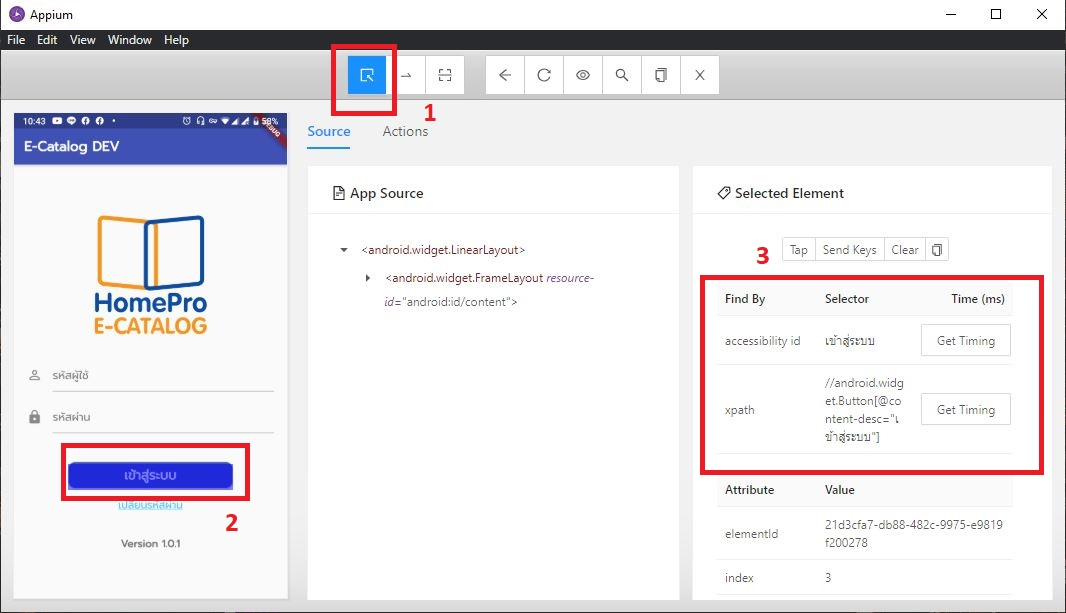
\includegraphics[width=1\textwidth]{xpathway}
        \caption{การดูค่า Element ด้วย Appium}\label{xpathway}
    \end{figure}

    จากรูปที่ 3.1 จะเห็นได้ว่าเมื่อชี้ที่ภาพในหมายเลข 2 จะปรากฎช่องด้านขวาซึ่งเป็นชื่อและค่าของ Element ที่อยู่ในช่องด้านขวาในหมายเลข 3 นำมาใช้งานต่อ

    \begin{figure}[H]
        \centering
        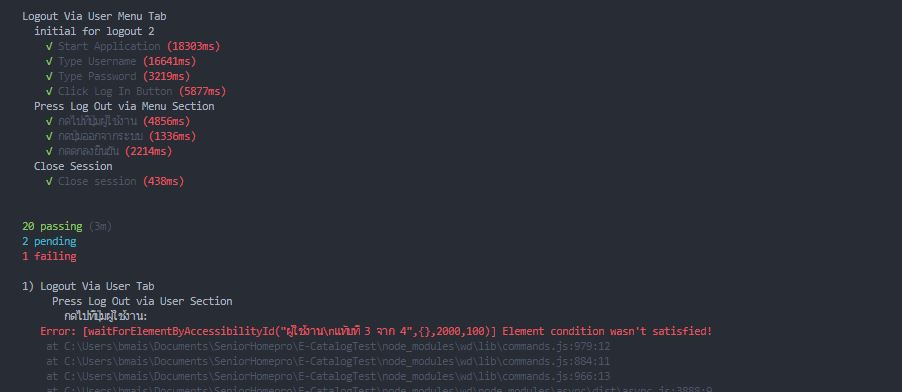
\includegraphics[width=1\textwidth]{output1}
        \caption{ตัวอย่างการแสดงผลของการทดสอบ}
        \label{result}
    \end{figure}

    จากรูป 3.2 เป็นรูปสรุปผลการทดสอบว่ามีผ่านจำนวนทั้งหมดเท่าไหร่ ผิดผลาด (Test Fail) เท่าไร่และทำไมถึงผิดพลาด        

    \begin{figure}[H]
        \centering
        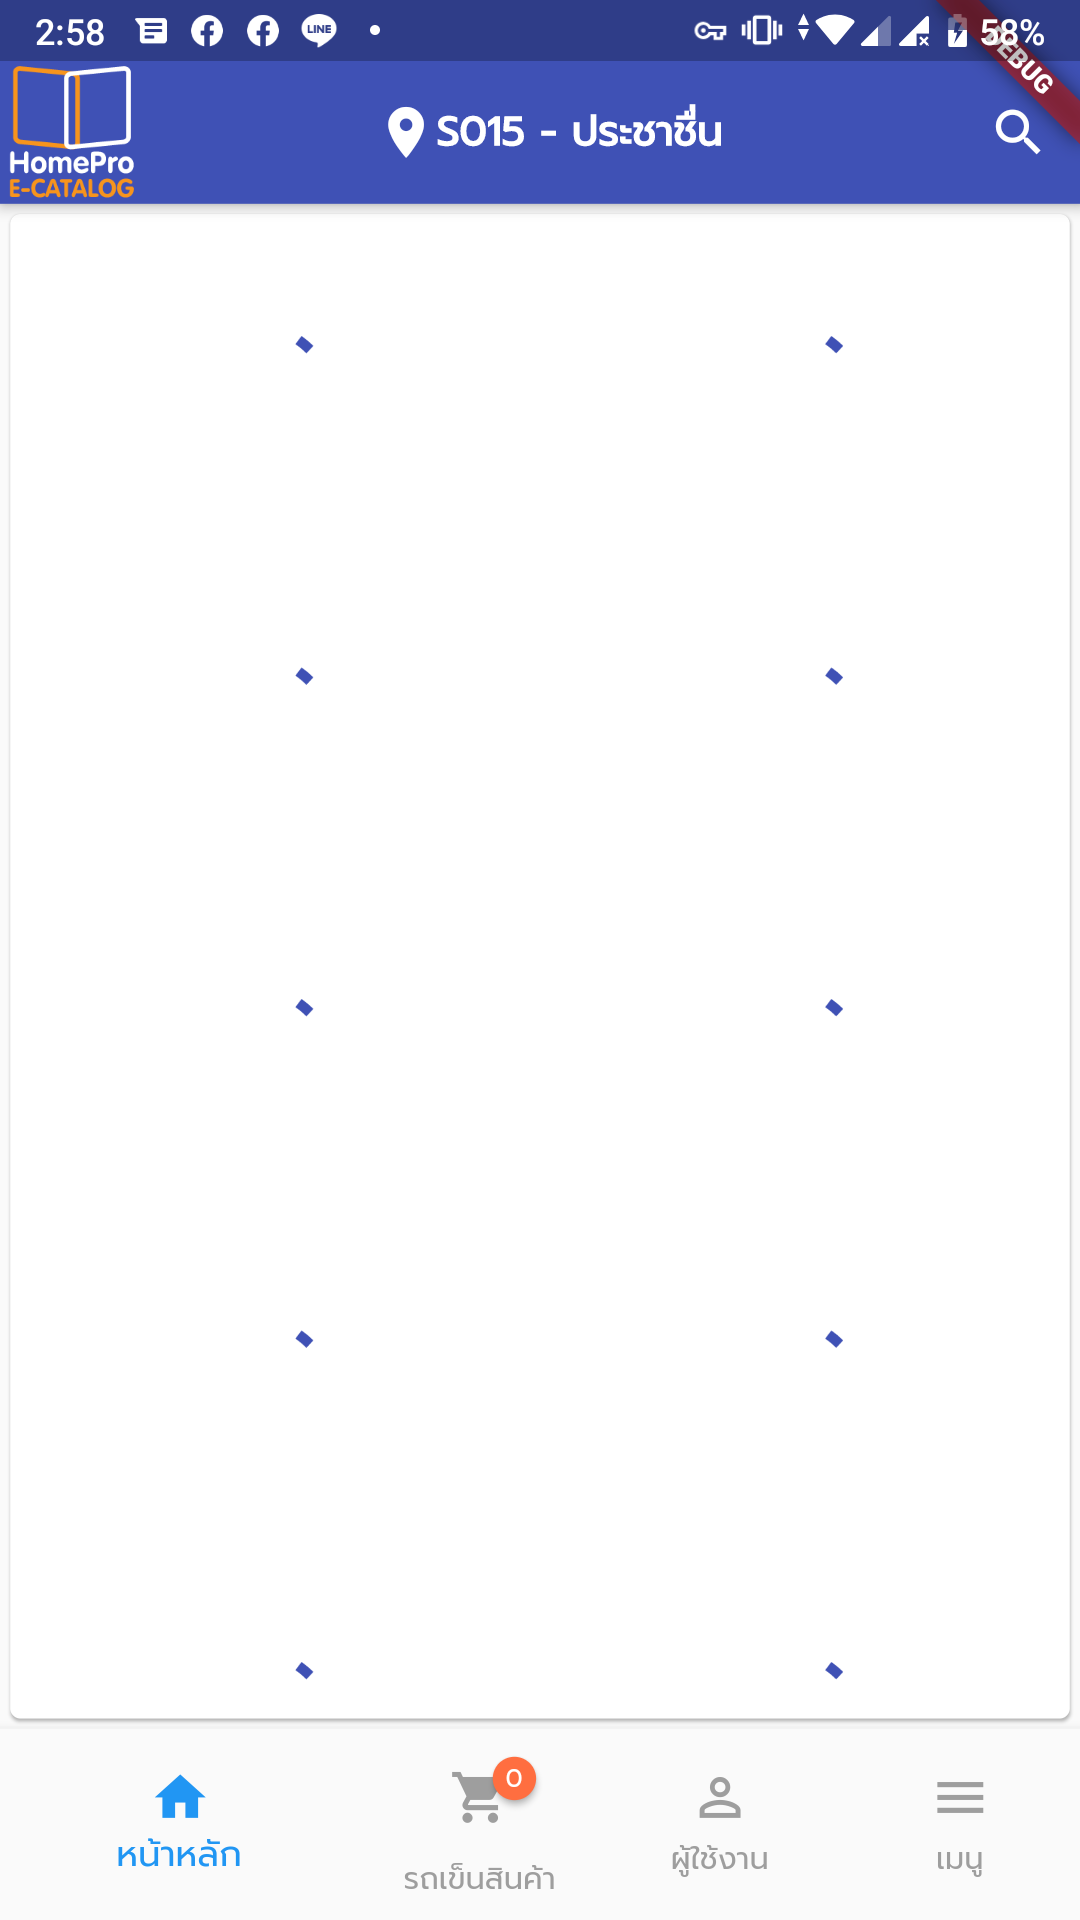
\includegraphics[width=0.35\textwidth]{1}
        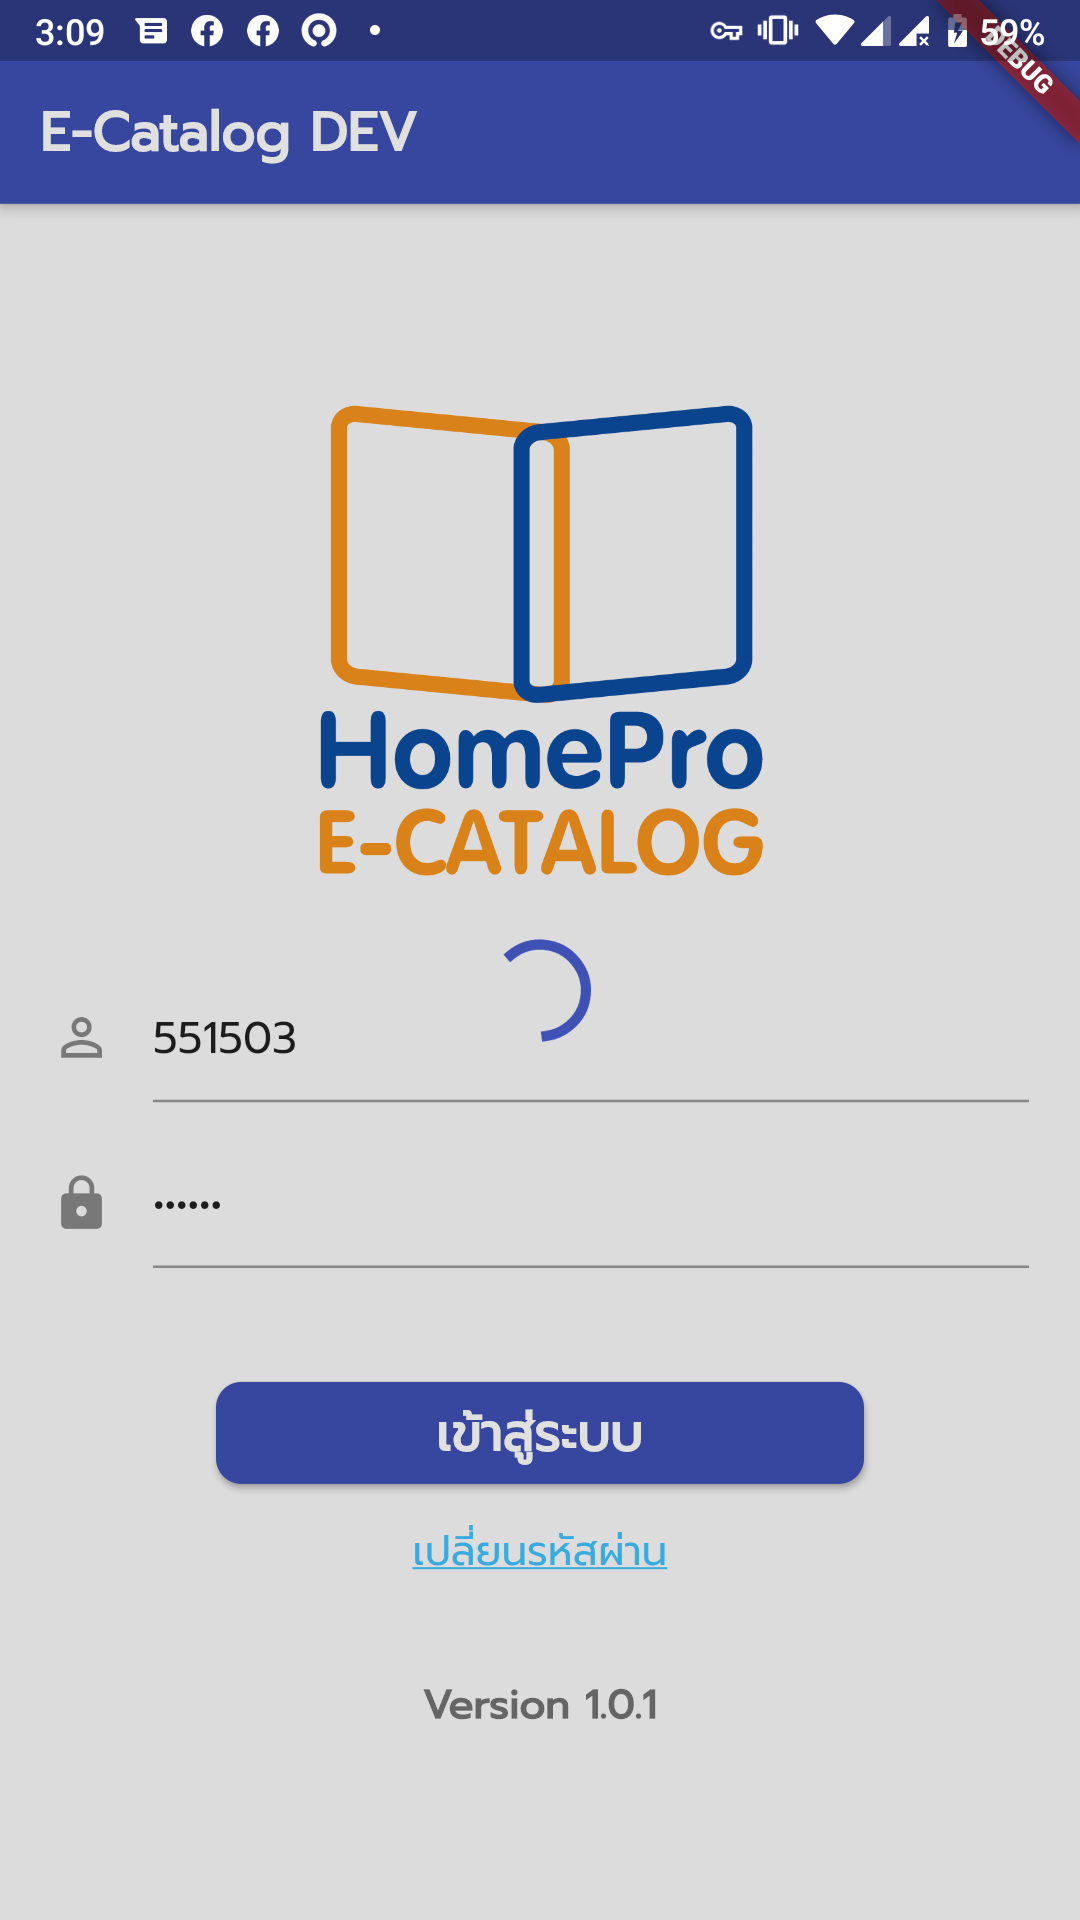
\includegraphics[width=0.35\textwidth]{2}
        \caption{ตัวอย่างการบันทึกหน้าจอเมื่อผิดผลาด}
        \label{errorPic}
    \end{figure}

    จากรูป 3.3 เป็นรูปที่เกิดจากการบันทึกหน้าจอเมื่อเจอข้อผิดผลาด (Test Fail) ดังตัวอย่างแสดงถึงเวลาที่หมดในการรอหน้าจอแสดงผลหรือใช้เวลาเกินกำหนดเป็นต้น

    \begin{longtable}{|l|l|}
        \caption{ตารางข้อเปรียบเทียบการทดสอบด้วยการจับ Element บนหน้าจอโดยไม่ต้องแก้ไขที่ Source Code}\\ 
        \hline
        \textbf{ข้อดี} & \textbf{ข้อเสีย} \endfirsthead 
        \hline
        \begin{tabular}[c]{@{}l@{}}สามารถจับ Element\\ได้โดยที่ไม่ต้อง\\ตามไปแก้ ที่ Source Code\end{tabular} & \begin{tabular}[c]{@{}l@{}}มีโอกาสที่ ลำดับของ \\Element \\จะคลาดเคลื่อน\\ตามขนาดโทรศัพท์\end{tabular}  \\ 
        \hline
        \begin{tabular}[c]{@{}l@{}}เปรียบเสมือนโทรศัพท์\\แสดงคีย์บอร์ดและกดได้\end{tabular}                   & \begin{tabular}[c]{@{}l@{}}บางคำสั่งอาจไม่รองรับการ\\ใช้งานกับ \\Appium ในคนละเวอร์ชัน\end{tabular}     \\
        \hline
    \end{longtable}

    \newpage
    \subsection{หน้า Log-in : กรอกรหัสพนักงาน และ รหัสผ่าน ถูกต้อง}
        \begin{longtable}{|l|l|l|} 
            \caption{ขอบเขตเหตุการณ์ Log-in ถูกต้อง} \\
            \hline
            \textbf{ลำดับ} & \textbf{เหตุการณ์ในการทดสอบ} & \textbf{ผลลัพธ์ในการทดสอบ}  \endfirsthead 
            \hline
            1              & กรอก username                & PASS                        \\ 
            \hline
            2              & กรอก password                & PASS                        \\ 
            \hline
            3              & กดปุ่ม login                 & PASS                        \\ 
            \hline
            4              & รอผลหน้าถัดไป                & PASS                        \\
            \hline
        \end{longtable}

        \begin{figure}[H]
            \centering
            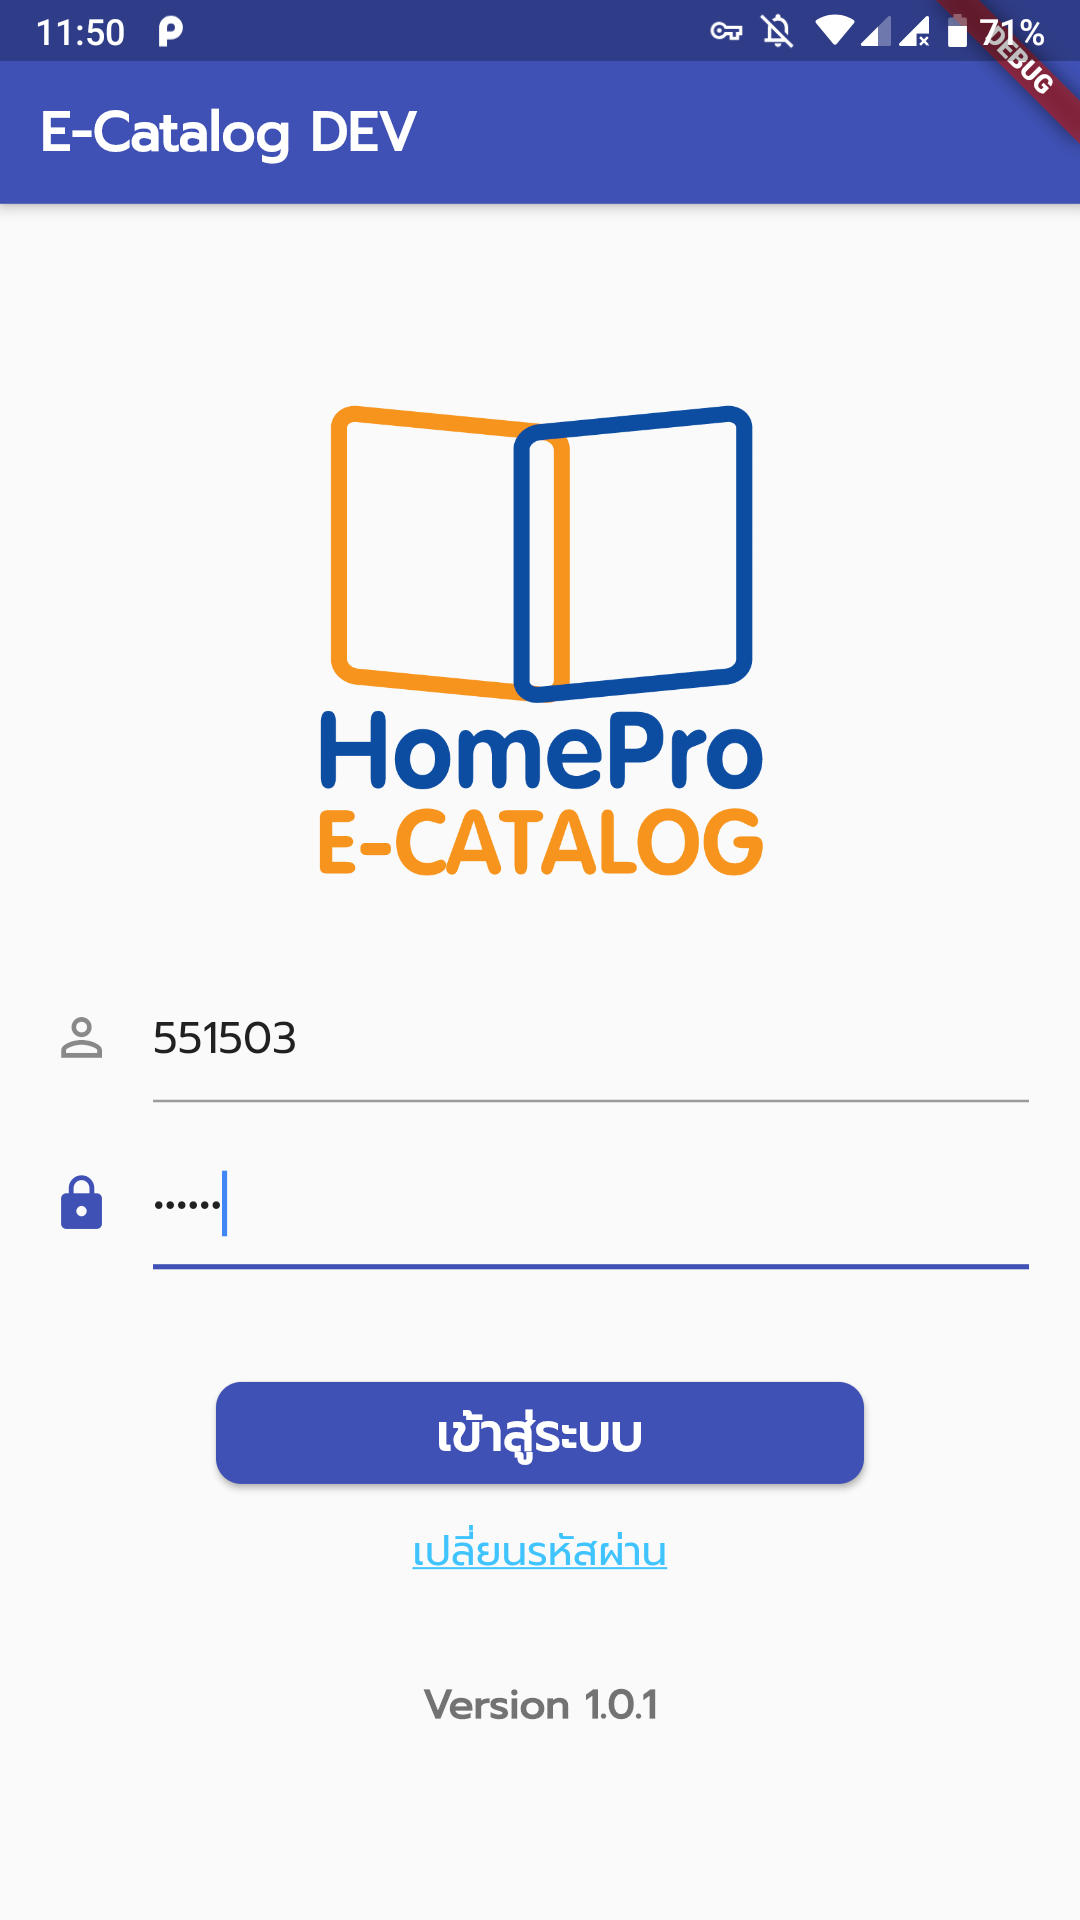
\includegraphics[width=0.35\textwidth]{loginPass2}
            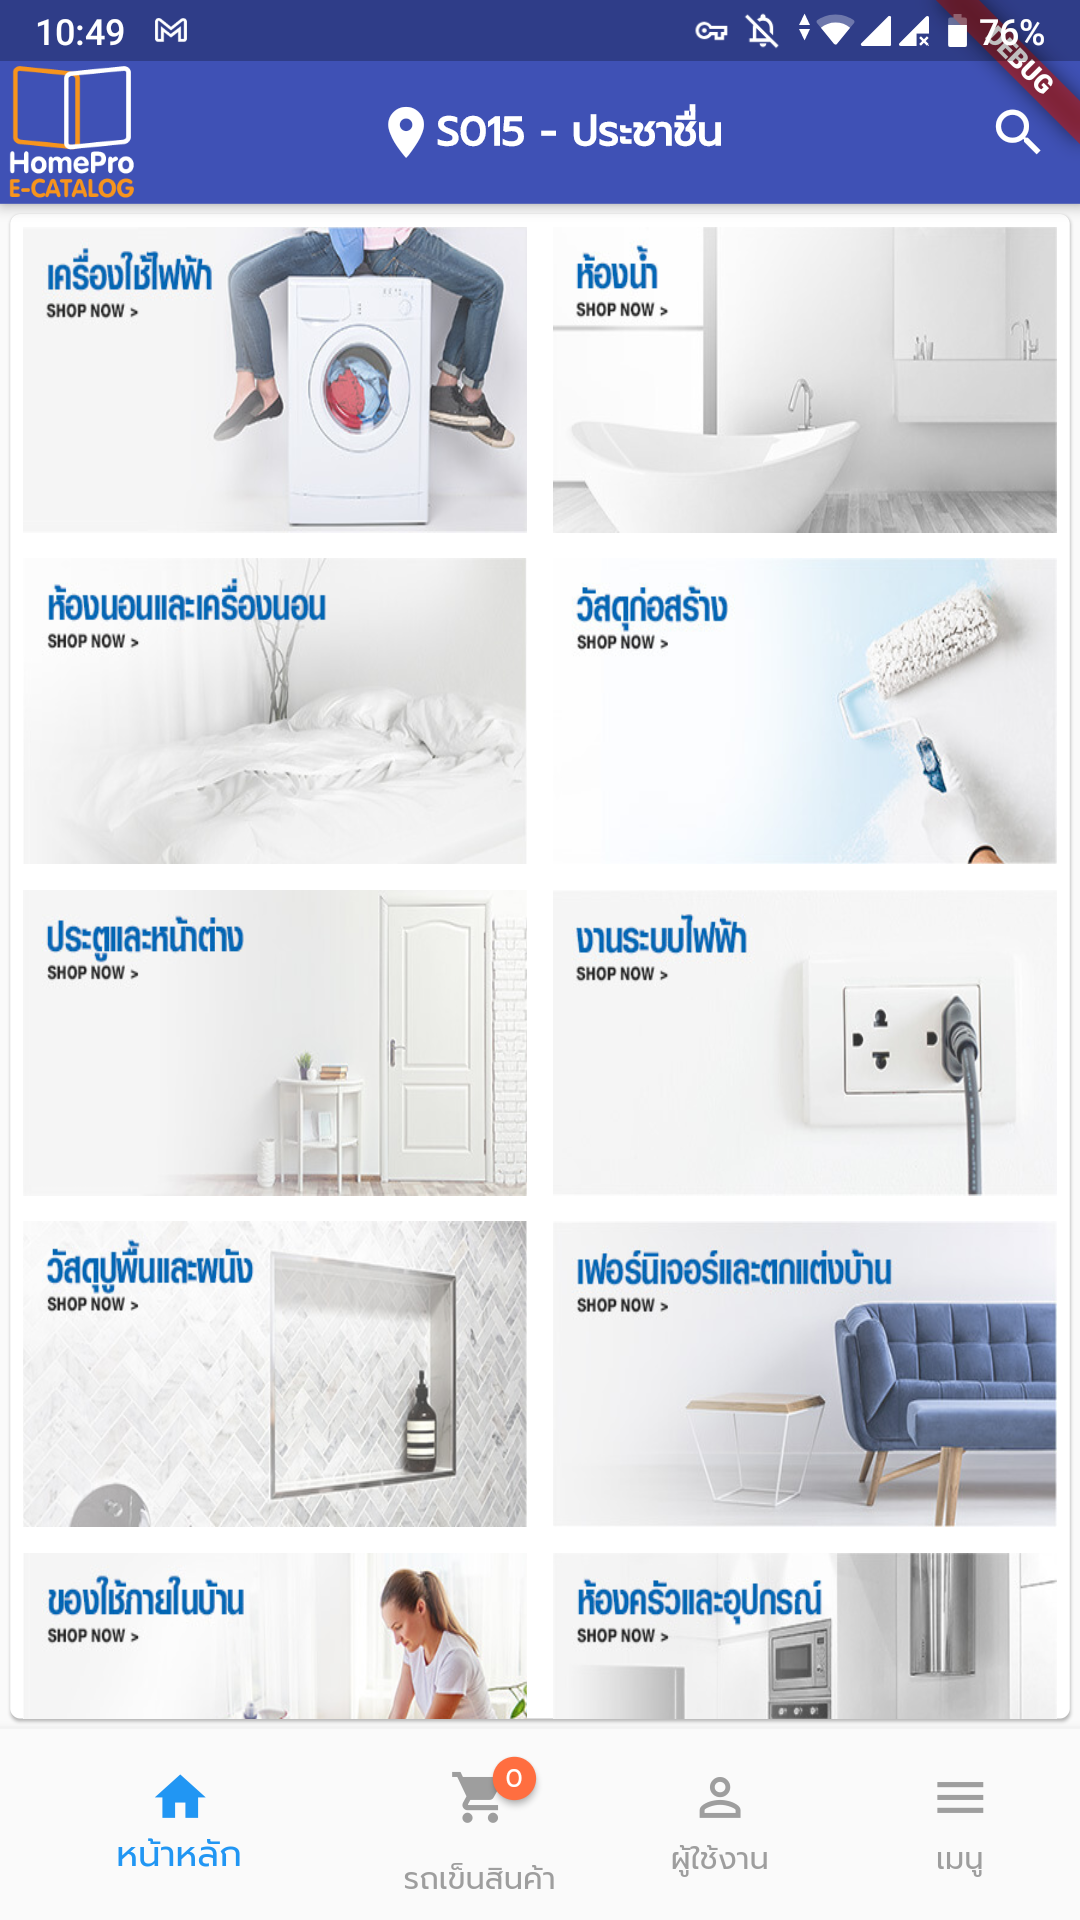
\includegraphics[width=0.35\textwidth]{loginPass3}
            \caption{ตัวอย่างเหตุการณ์ Log-in ถูกต้อง}
            \label{Fig:25}
        \end{figure}
    
    \newpage
    \subsection{หน้า Log-in : กรอกรหัสพนักงาน หรือ รหัสผ่าน ไม่ถูกต้อง}
        \begin{longtable}{|l|l|l|} 
            \caption{ขอบเขตเหตุการณ์ Log-in ไม่ถูกต้อง (กรอก usename ไม่ถูกต้อง)} \\
            \hline
            \textbf{ลำดับ} & \textbf{เหตุการณ์ในการทดสอบ} & \textbf{ผลลัพธ์ในการทดสอบ}  \endfirsthead 
            \hline
            1              & กรอก username ผิด               & PASS                        \\ 
            \hline
            2              & กรอก password                & PASS                        \\ 
            \hline
            3              & กดปุ่ม login                 & PASS                        \\ 
            \hline
            4              & ไม่พบข้อมูลผู้ใช้งาน                & PASS                        \\
            \hline
        \end{longtable}

        \begin{longtable}{|l|l|l|}
            \caption{ขอบเขตเหตุการณ์ Log-in ไม่ถูกต้อง (กรอก password ไม่ถูกต้อง)} \\ 
            \hline
            \textbf{ลำดับ} & \textbf{เหตุการณ์ในการทดสอบ} & \textbf{ผลลัพธ์ในการทดสอบ}  \endfirsthead 
            \hline
            1              & กรอก username               & PASS                        \\ 
            \hline
            2              & กรอก password ผิด                & PASS                        \\ 
            \hline
            3              & กดปุ่ม login                 & PASS                        \\ 
            \hline
            4              & รหัสผ่านไม่ถูกต้อง                & PASS                        \\
            \hline
        \end{longtable}

        \begin{figure}[H]
            \centering
            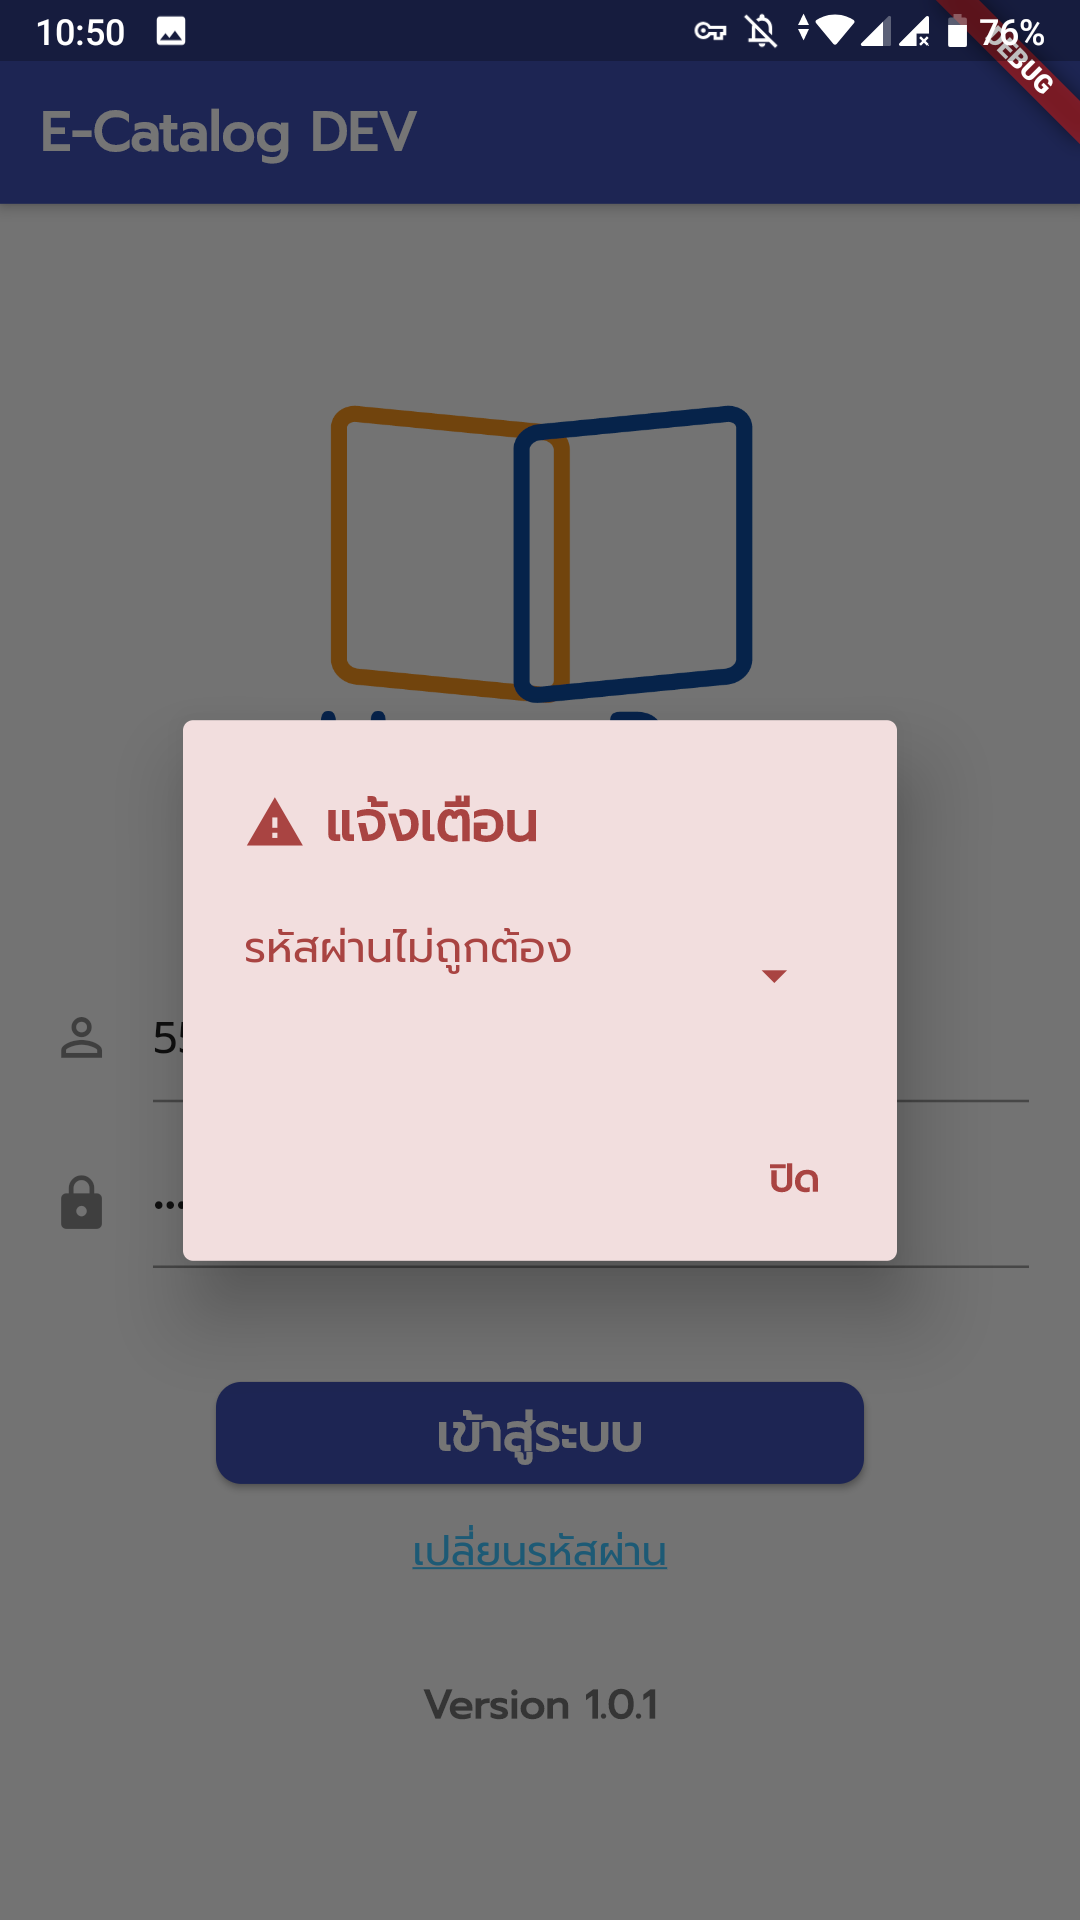
\includegraphics[width=0.35\textwidth]{loginFail1}
            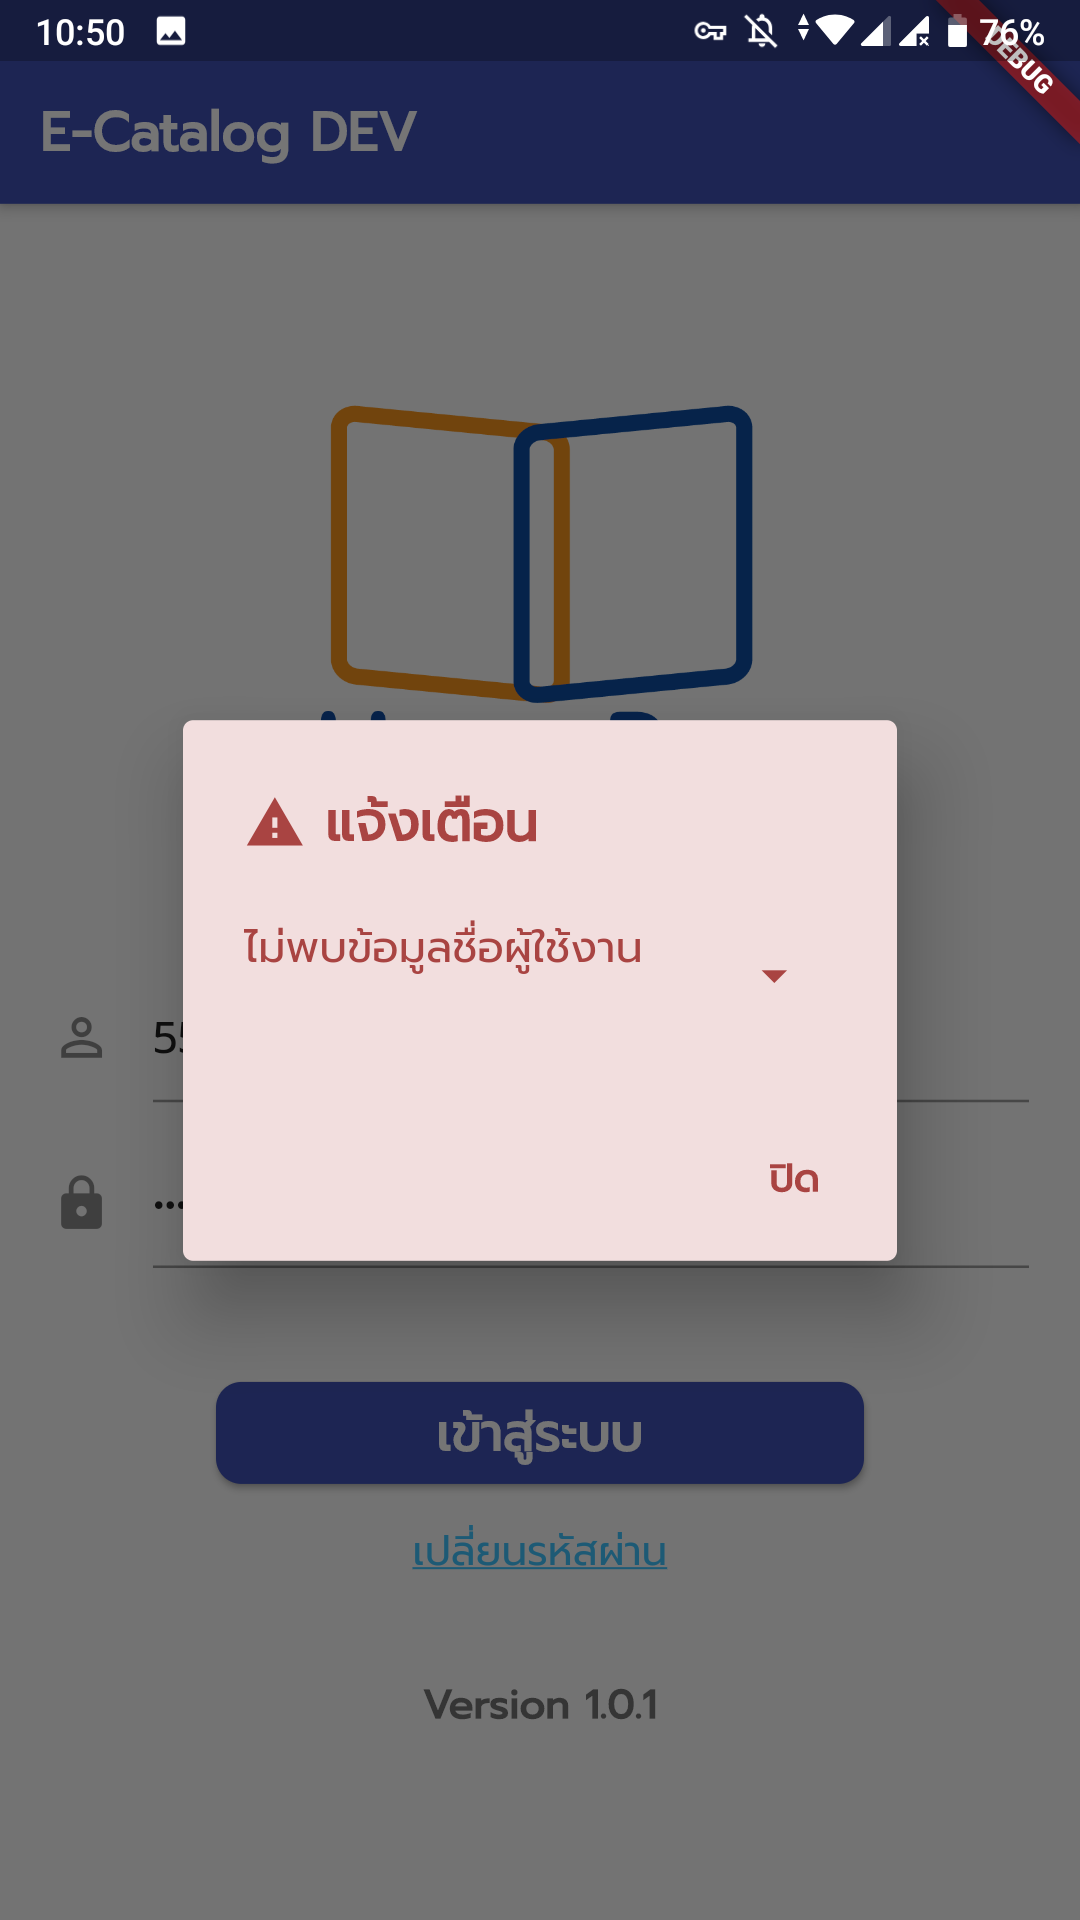
\includegraphics[width=0.35\textwidth]{loginFail2}
            \caption{ตัวอย่างเหตุการณ์ Log-in ถูกต้อง}
            \label{Fig:26}
        \end{figure}

    \newpage
    \subsection{ออกจากระบบ : ต้องการออกจากระบบด้วยแทบ "ผู้ใช้งาน" ใน BottomNavigationBar}

    \begin{longtable}{|l|l|l|}
        \caption{ขอบเขตเหตุการณ์ ออกจากระบบด้วยแทบ "ผู้ใช้งาน" ใน BottomNavigationBar} \\ 
        \hline
        \textbf{ลำดับ} & \textbf{เหตุการณ์ในการทดสอบ} & \textbf{ผลลัพธ์ในการทดสอบ}  \endfirsthead 
        \hline
        1              & ทำการ Log-in               & PASS                        \\ 
        \hline
        2              & กดไปที่ปุ่มผู้ใช้งาน                & PASS                        \\ 
        \hline
        3              & กดปุ่มออกจากระบบ                & PASS                        \\ 
        \hline
        4              & กดตกลงยืนยันและไปหน้า log-in     & PASS                        \\
        \hline
    \end{longtable}

    \begin{figure}[H]
        \centering
        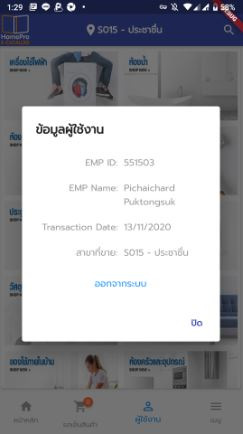
\includegraphics[width=0.35\textwidth]{logout1_2}
        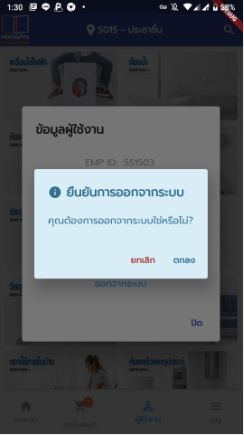
\includegraphics[width=0.35\textwidth]{logout1_3}
        \caption{ตัวอย่างเหตุการณ์ ออกจากระบบด้วยแทบ "ผู้ใช้งาน" ใน BottomNavigationBar}
        \label{Fig:27}
    \end{figure}

    \newpage
    \subsection{ออกจากระบบ : ต้องการออกจากระบบด้วยแทบ "เมนู" ใน BottomNavigationBar}

    \begin{longtable}{|l|l|l|} 
        \caption{ขอบเขตเหตุการณ์ ออกจากระบบด้วยแทบ "เมนู" ใน BottomNavigationBar} \\
        \hline
        \textbf{ลำดับ} & \textbf{เหตุการณ์ในการทดสอบ} & \textbf{ผลลัพธ์ในการทดสอบ}  \endfirsthead 
        \hline
        1              & ทำการ Log-in               & PASS                        \\ 
        \hline
        2              & กดไปที่ปุ่มเมนู               & PASS                        \\ 
        \hline
        3              & กดปุ่มออกจากระบบ                & PASS                        \\ 
        \hline
        4              & กดตกลงยืนยันและไปหน้า log-in     & PASS                        \\
        \hline
    \end{longtable}

    \begin{figure}[H]
        \centering
        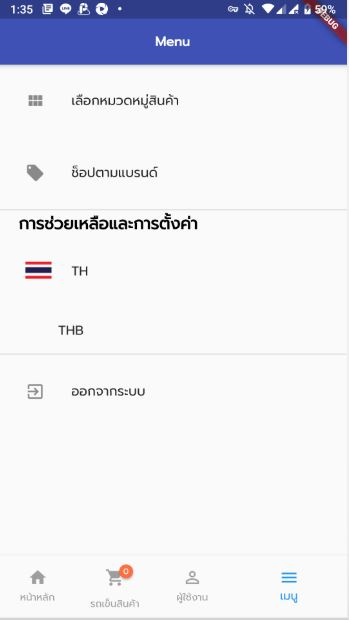
\includegraphics[width=0.35\textwidth]{logout2}
        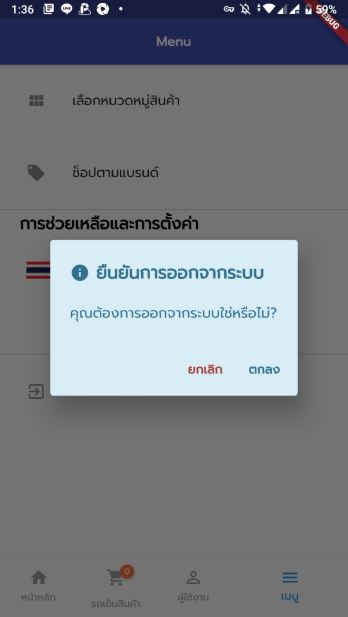
\includegraphics[width=0.35\textwidth]{logout2_1}
        \caption{ตัวอย่างเหตุการณ์ ออกจากระบบด้วยแทบ "เมนู" ใน BottomNavigationBar}
        \label{Fig:28}
    \end{figure}

    \newpage
    \subsection{หน้าหลัก - รายละเอียดสินค้า (Detail) : ตรวจสอบรายละเอียดของสินค้า}

    สามารถแบ่งได้เป็น 2 ประเภทคือ รายละเอียดสินค้า ราคาธรรมดาและสินค้าราคาโปรโมชัน

    \begin{longtable}{|l|l|l|}
        \caption{ขอบเขตเหตุการณ์ รายละเอียดสินค้า (Detail) ตรวจสอบรายละเอียดของสินค้าธรรมดา} \\ 
        \hline
        \textbf{ลำดับ} & \textbf{เหตุการณ์ในการทดสอบ} & \textbf{ผลลัพธ์ในการทดสอบ}  \endfirsthead 
        \hline
        1              & ทำการ Log-in               & PASS                        \\ 
        \hline
        2              & กดไปที่หมวดเครื่องใช้ไฟฟ้า               & PASS                        \\ 
        \hline
        3              & กดปุ่มหมวดย่อยไปที่เครื่องเตรียมอาหาร                & PASS                        \\ 
        \hline
        4              & เลือกสินค้าธรรมดา     & PASS                        \\
        \hline
        5              & เช็คแบรนสินค้า     & PASS                        \\
        \hline
        6              & เช็คชื่อสินค้า     & PASS                        \\
        \hline
        7              & เช็ครหัสสินค้า     & PASS                        \\
        \hline
        8              & เช็คราคาแบบธรรมดา     & PASS                        \\
        \hline
    \end{longtable}

    \begin{longtable}{|l|l|l|} 
        \caption{ขอบเขตเหตุการณ์ รายละเอียดสินค้า (Detail) ตรวจสอบรายละเอียดของสินค้ามีโปรโมชัน} \\
        \hline
        \textbf{ลำดับ} & \textbf{เหตุการณ์ในการทดสอบ} & \textbf{ผลลัพธ์ในการทดสอบ}  \endfirsthead 
        \hline
        1              & ทำการ Log-in               & PASS                        \\ 
        \hline
        2              & กดไปที่หมวดเครื่องใช้ไฟฟ้า               & PASS                        \\ 
        \hline
        3              & กดปุ่มหมวดย่อยไปที่เครื่องเตรียมอาหาร                & PASS                        \\ 
        \hline
        4              & เลือกสินค้าธรรมดา     & PASS                        \\
        \hline
        5              & เช็คแบรนสินค้า     & PASS                        \\
        \hline
        6              & เช็คชื่อสินค้า     & PASS                        \\
        \hline
        7              & เช็ครหัสสินค้า     & PASS                        \\
        \hline
        8              & เช็คราคาแบบธรรมดา     & PASS                        \\
        \hline
        9              & เช็คราคาแบบโปรโมชั่น     & PASS                        \\
        \hline
    \end{longtable}

    \begin{figure}[H]
        \centering
        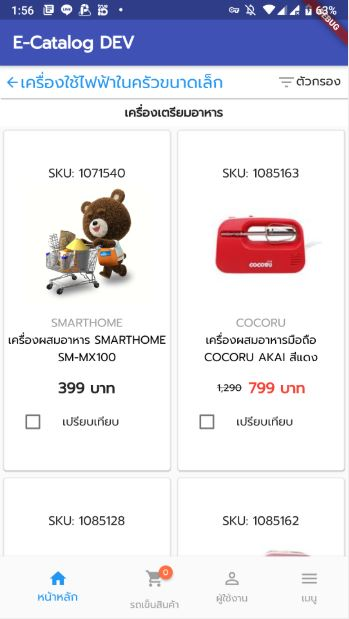
\includegraphics[width=0.35\textwidth]{detail1_2.JPG}
        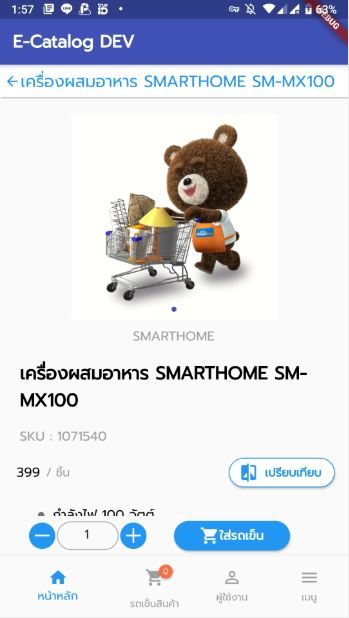
\includegraphics[width=0.35\textwidth]{detail1_3.JPG}
        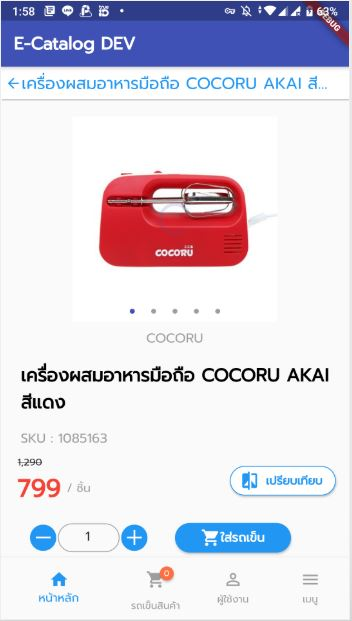
\includegraphics[width=0.35\textwidth]{detail1_4.JPG}
        \caption{ตัวอย่างเหตุการณ์ รายละเอียดสินค้า (Detail) ตรวจสอบรายละเอียดของสินค้า}
        \label{Fig:51}
    \end{figure}

    \newpage
    \subsection{หน้าหลัก - รายละเอียดสินค้า (Detail) : ปุ่มเปรียบเทียบ หน้า Detail}

    \begin{longtable}{|l|l|l|} 
        \caption{ขอบเขตเหตุการณ์ รายละเอียดสินค้า (Detail) ปุ่มเปรียบเทียบ หน้า Detail} \\
        \hline
        \textbf{ลำดับ} & \textbf{เหตุการณ์ในการทดสอบ} & \textbf{ผลลัพธ์ในการทดสอบ}  \endfirsthead 
        \hline
        1              & ทำการ Log-in               & PASS                        \\ 
        \hline
        2              & เลือกสินค้า               & PASS                        \\ 
        \hline
        3              & กดปุ่มเปรียบเทียบ                & PASS                        \\ 
        \hline
        4              & เช็คว่ามีสินค้าในช่องเปรียบเทียบ     & PASS                        \\
        \hline
    \end{longtable}

    \begin{figure}[H]
        \centering
        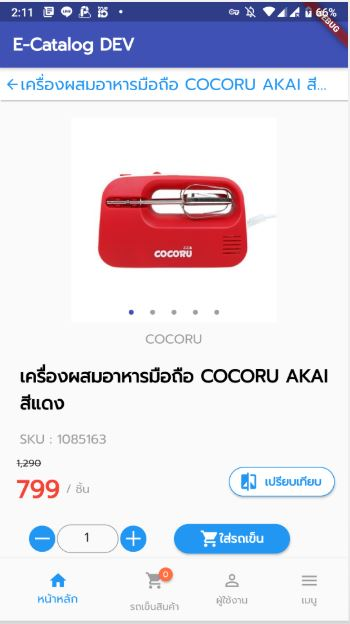
\includegraphics[width=0.35\textwidth]{detailCom1.JPG}
        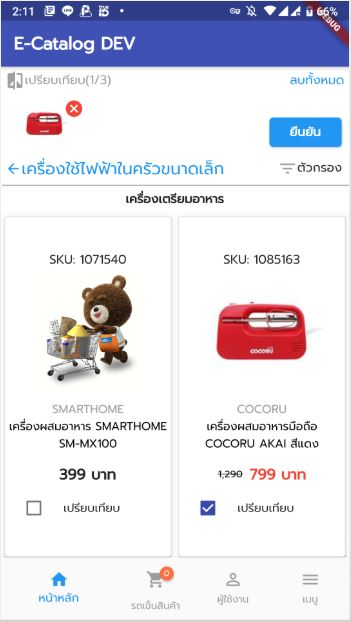
\includegraphics[width=0.35\textwidth]{deatilCom2.JPG}
        \caption{ตัวอย่างเหตุการณ์ รายละเอียดสินค้า (Detail) ปุ่มเปรียบเทียบ หน้า Detail}
        \label{Fig:59}
    \end{figure}


    \subsection{หน้าหลัก - รายละเอียดสินค้า (Detail) : แถบรายละเอียดสินค้า}

    \begin{longtable}{|l|l|l|}
        \caption{ขอบเขตเหตุการณ์ รายละเอียดสินค้า (Detail) แถบรายละเอียดสินค้า} \\ 
        \hline
        \textbf{ลำดับ} & \textbf{เหตุการณ์ในการทดสอบ} & \textbf{ผลลัพธ์ในการทดสอบ}  \endfirsthead 
        \hline
        1              & ทำการ Log-in               & PASS                        \\ 
        \hline
        2              & เลือกสินค้า               & PASS                        \\ 
        \hline
        3              & ไปหาเช็คแถบรายละเอียดสินค้ากดปุ่มเพิ่มเติม       & PASS                        \\ 
        \hline
        4              & มีรายละเอียดสินค้า     & PASS                        \\
        \hline
    \end{longtable}

    \begin{figure}[H]
        \centering
        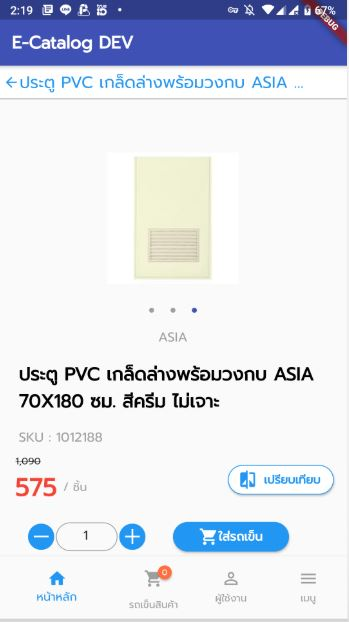
\includegraphics[width=0.35\textwidth]{deatilInfo1}
        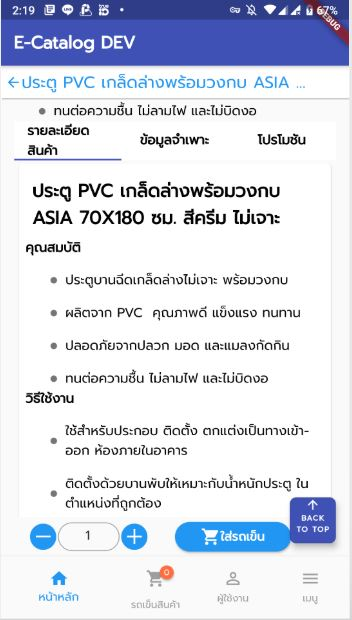
\includegraphics[width=0.35\textwidth]{detailInfo1_2}
        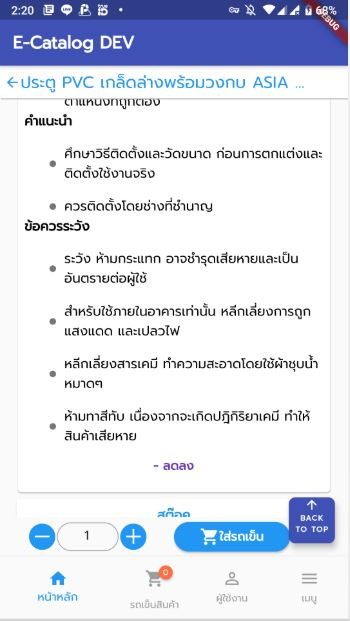
\includegraphics[width=0.35\textwidth]{detailInfo1_3}
        \caption{ตัวอย่างเหตุการณ์ รายละเอียดสินค้า (Detail) แถบรายละเอียดสินค้า}
        \label{Fig:29}
    \end{figure}

    \newpage
    \subsection{หน้าหลัก - รายละเอียดสินค้า (Detail) : แถบข้อมูลจำเพาะ}

    \begin{longtable}{|l|l|l|}
        \caption{ขอบเขตเหตุการณ์ รายละเอียดสินค้า (Detail) แถบข้อมูลจำเพาะ} \\ 
        \hline
        \textbf{ลำดับ} & \textbf{เหตุการณ์ในการทดสอบ} & \textbf{ผลลัพธ์ในการทดสอบ}  \endfirsthead 
        \hline
        1              & ทำการ Log-in               & PASS                        \\ 
        \hline
        2              & เลือกสินค้า               & PASS                        \\ 
        \hline
        3              & ไปยังหมวดข้อมูลจำเพาะ       & PASS                        \\ 
        \hline
        4              & เช็ค Brand     & PASS                        \\
        \hline
        5              & เช็ค Color     & PASS                        \\
        \hline
        6              & เช็ค ประเภทหน้าบาน     & PASS                        \\
        \hline
        7              & เช็ค ผิวเคลือบ     & PASS                        \\
        \hline
        8              & เช็ค การขึ้นรูป     & PASS                        \\
        \hline
        9              & เช็ค ลายหน้าบาน     & PASS                        \\
        \hline
        10              & เช็ค Material     & PASS                        \\
        \hline
        11             & เช็ค Size     & PASS                        \\
        \hline
    \end{longtable}

    \begin{figure}[H]
        \centering
        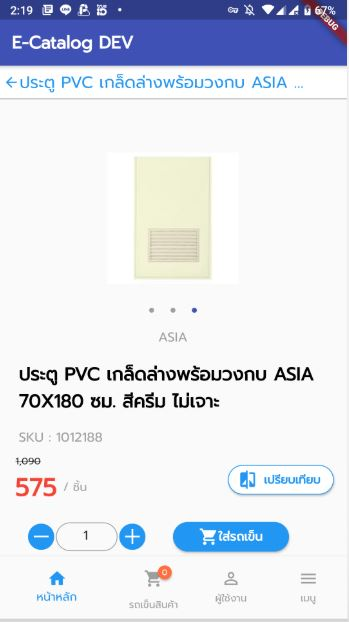
\includegraphics[width=0.35\textwidth]{deatilInfo1}
        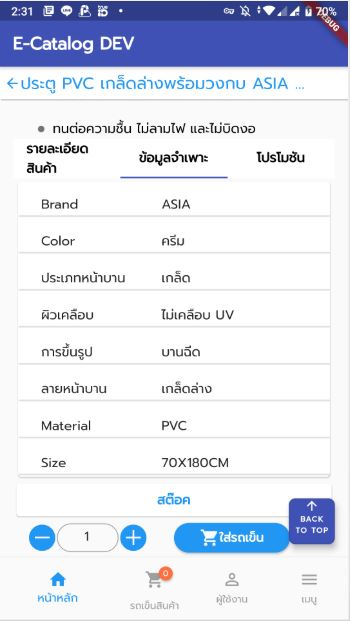
\includegraphics[width=0.35\textwidth]{detailInfo2.JPG}
        \caption{ตัวอย่างเหตุการณ์ รายละเอียดสินค้า (Detail) แถบข้อมูลจำเพาะ}
        \label{Fig:30}
    \end{figure}

    \newpage
    \subsection{หน้าหลัก - รายละเอียดสินค้า (Detail) : แถบโปรโมชั่นหน้าหลัก}

    \begin{longtable}{|l|l|l|} 
        \caption{ขอบเขตเหตุการณ์ รายละเอียดสินค้า (Detail) แถบโปรโมชั่นหน้าหลัก} \\
        \hline
        \textbf{ลำดับ} & \textbf{เหตุการณ์ในการทดสอบ} & \textbf{ผลลัพธ์ในการทดสอบ}  \endfirsthead 
        \hline
        1              & ทำการ Log-in               & PASS                        \\ 
        \hline
        2              & เลือกสินค้า               & PASS                        \\ 
        \hline
        3              & ไปยังหมวดโปรโมชัน       & PASS                        \\ 
        \hline
        4              & เช็ค โปรโมชัน 1 อันเป็นตัวอย่างว่าข้อมูลเข้า     & PASS                        \\
        \hline
    \end{longtable}

    \begin{figure}[H]
        \centering
        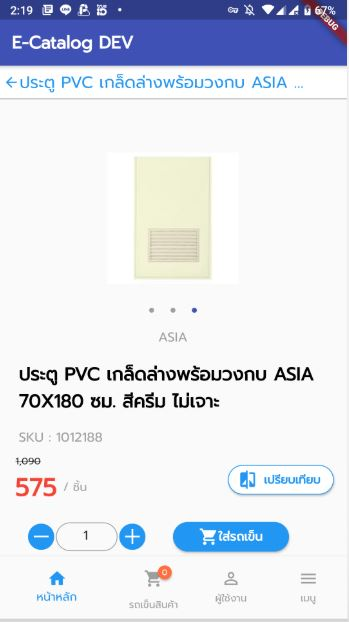
\includegraphics[width=0.35\textwidth]{deatilInfo1}
        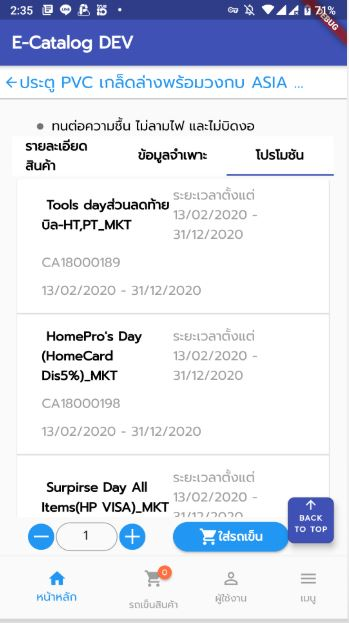
\includegraphics[width=0.35\textwidth]{detailPromotion}
        \caption{ตัวอย่างเหตุการณ์ รายละเอียดสินค้า (Detail) แถบโปรโมชั่นหน้าหลัก}
        \label{Fig:31}
    \end{figure}

    \newpage
    \subsection{หน้าหลัก - รายละเอียดสินค้า (Detail) : ปุ่ม สต๊อกสินค้า}

    \begin{longtable}{|l|l|l|} 
        \caption{ขอบเขตเหตุการณ์ รายละเอียดสินค้า (Detail) ปุ่ม สต๊อกสินค้า} \\
        \hline
        \textbf{ลำดับ} & \textbf{เหตุการณ์ในการทดสอบ} & \textbf{ผลลัพธ์ในการทดสอบ}  \endfirsthead 
        \hline
        1              & ทำการ Log-in               & PASS                        \\ 
        \hline
        2              & เลือกสินค้า               & PASS                        \\ 
        \hline
        3              & ไปหาและกดปุ่มสต๊อค       & PASS                        \\ 
        \hline
        4              & มีรายสาขาที่ของผู้ใช้ขึ้นก่อน     & PASS                        \\
        \hline
        5              & เป็นสาขา DC01     & PASS                        \\
        \hline
        6              & เป็นสาขา DC02     & PASS                        \\
        \hline
    \end{longtable}

    \begin{figure}[H]
        \centering
        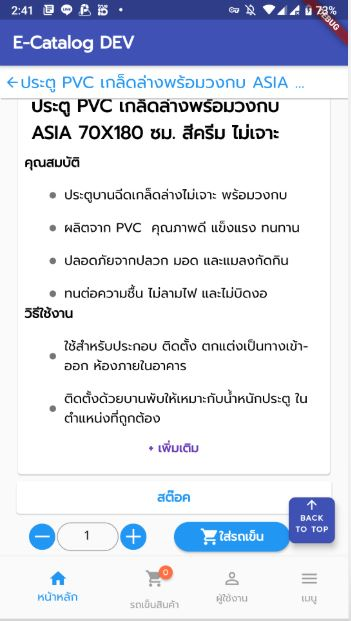
\includegraphics[width=0.35\textwidth]{stock1_2}
        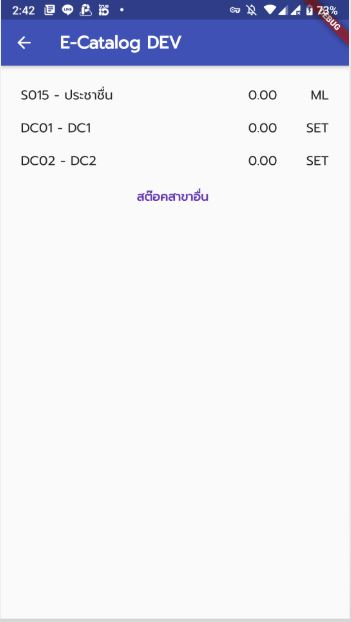
\includegraphics[width=0.35\textwidth]{stock1_3}
        \caption{ตัวอย่างเหตุการณ์ รายละเอียดสินค้า (Detail) ปุ่ม สต๊อกสินค้า}
        \label{Fig:32}
    \end{figure}

    \newpage
    \subsection{หน้าหลัก - รายละเอียดสินค้า (Detail) : ปุ่ม สต๊อกสินค้าเพิ่มเติม}

    \begin{longtable}{|l|l|l|} 
        \caption{ขอบเขตเหตุการณ์ รายละเอียดสินค้า (Detail) ปุ่ม สต๊อกสินค้าเพิ่มเติม} \\
        \hline
        \textbf{ลำดับ} & \textbf{เหตุการณ์ในการทดสอบ} & \textbf{ผลลัพธ์ในการทดสอบ}  \endfirsthead 
        \hline
        1              & ทำการ Log-in               & PASS                        \\ 
        \hline
        2              & เลือกสินค้า               & PASS                        \\ 
        \hline
        3              & ไปหาและกดปุ่มสต๊อค       & PASS                        \\ 
        \hline
        4              & กดไปที่สต๊อคสาขาอื่น     & PASS                        \\
        \hline
        5              & เช็คลำดับสต๊อคจากสาขามีมากไปน้อย     & PASS                        \\
        \hline
    \end{longtable}

    \begin{figure}[H]
        \centering
        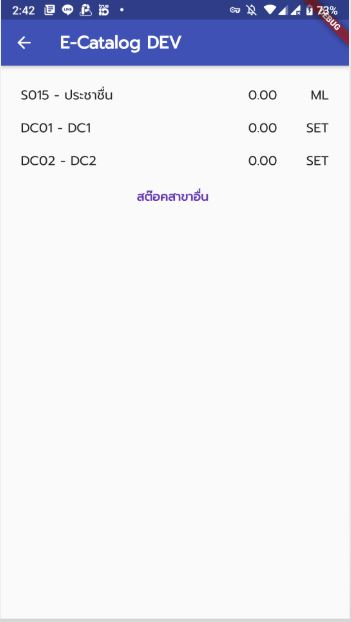
\includegraphics[width=0.35\textwidth]{stock1_3}
        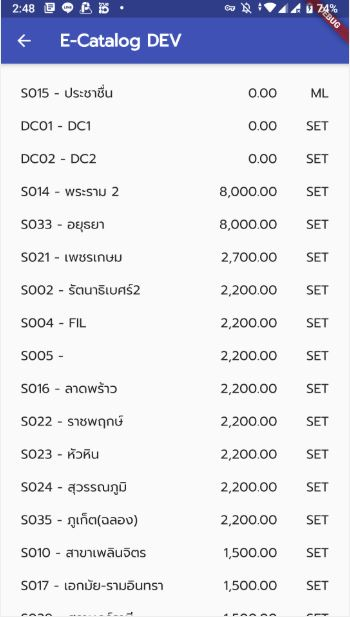
\includegraphics[width=0.35\textwidth]{stockMore.JPG}
        \caption{ตัวอย่างเหตุการณ์ รายละเอียดสินค้า (Detail) ปุ่ม สต๊อกสินค้าเพิ่มเติม}
        \label{Fig:33}
    \end{figure}

    \newpage
    \subsection{หน้าจอเปรียบเทียบสินค้า : เปรียบเทียบ}

    \begin{longtable}{|l|l|l|} 
        \caption{ขอบเขตเหตุการณ์ เปรียบเทียบสินค้า} \\
        \hline
        \textbf{ลำดับ} & \textbf{เหตุการณ์ในการทดสอบ} & \textbf{ผลลัพธ์ในการทดสอบ}  \endfirsthead 
        \hline
        1              & ทำการ Log-in               & PASS                        \\ 
        \hline
        2              & ไปยังหมวดหมู่ย่อย               & PASS                        \\ 
        \hline
        3              & กดเลือกปุ่มเปรียบเทียบสินค้า 3 ชิ้น       & PASS                        \\ 
        \hline
        4              & กดยืนยันการเปรียบเทียบ     & PASS                        \\
        \hline
        5              & เช็ค ความกว้าง     & PASS                        \\
        \hline
        6              & เช็ค ความลึก     & PASS                        \\
        \hline
        7              & เช็ค Material     & PASS                        \\
        \hline
        8              & เช็ค ระดับ     & PASS                        \\
        \hline
        9              & เช็ค อุปกรณ์เสริม     & PASS                        \\
        \hline
        10              & เช็ค ฺBrand     & PASS                        \\
        \hline
        11              & เช็ค ความสูง     & PASS                        \\
        \hline
        12              & เช็ค น้ำหนัก     & PASS                        \\
        \hline
        13              & เช็ค กำลังไฟ     & PASS                        \\
        \hline
        14              & เช็ค Size     & PASS                        \\
        \hline
        15              & เช็ค Color     & PASS                        \\
        \hline
    \end{longtable}

    \begin{figure}[H]
        \centering
        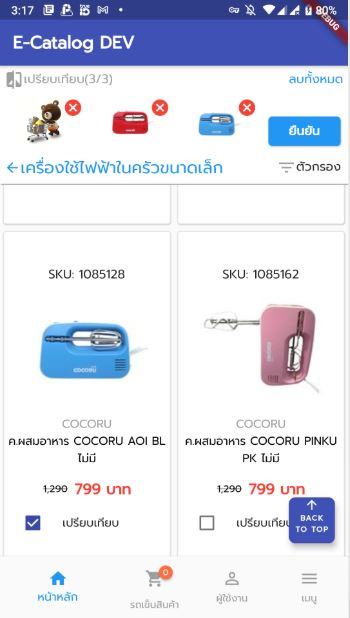
\includegraphics[width=0.35\textwidth]{compare1_2}
        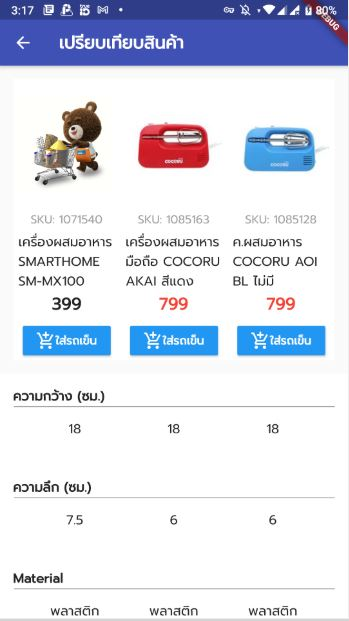
\includegraphics[width=0.35\textwidth]{compare1_3}
        \caption{ตัวอย่างเหตุการณ์ เปรียบเทียบสินค้า}
        \label{Fig:34}
    \end{figure}

    \newpage
    \subsection{หน้าจอเปรียบเทียบสินค้า : เปรียบเทียบมากกว่า 3 รายการ}

    \begin{longtable}{|l|l|l|} 
        \caption{ขอบเขตเหตุการณ์ เปรียบเทียบมากกว่า 3 รายการ} \\
        \hline
        \textbf{ลำดับ} & \textbf{เหตุการณ์ในการทดสอบ} & \textbf{ผลลัพธ์ในการทดสอบ}  \endfirsthead 
        \hline
        1              & ทำการ Log-in               & PASS                        \\ 
        \hline
        2              & ไปยังหมวดหมู่ย่อย               & PASS                        \\ 
        \hline
        3              & กดเลือกปุ่มเปรียบเทียบสินค้า 4 ชิ้น       & PASS                        \\ 
        \hline
        4              & แสดงจำนวนสินค้าเปรียบเทียบเกินกำหนด     & PASS                        \\
        \hline
    \end{longtable}

    \begin{figure}[H]
        \centering
        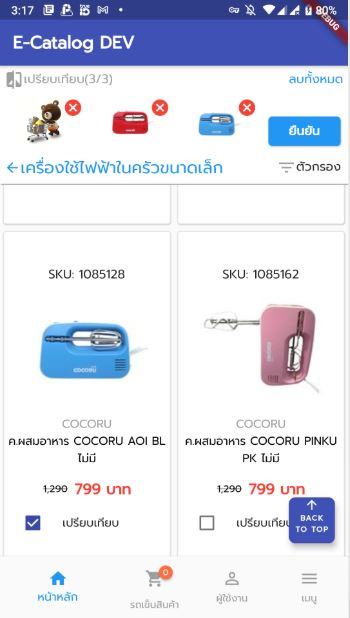
\includegraphics[width=0.35\textwidth]{compare1_2}
        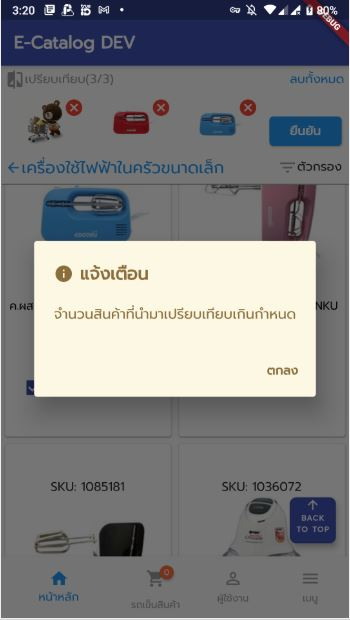
\includegraphics[width=0.35\textwidth]{compareMore}
        \caption{ตัวอย่างเหตุการณ์ เปรียบเทียบมากกว่า 3 รายการ}
        \label{Fig:35}
    \end{figure}

    \subsection{หน้าจอเปรียบเทียบสินค้า : ยกเลิกตัวที่เปรียบเทียบบางรายการ}

    \begin{longtable}{|l|l|l|}
        \caption{ขอบเขตเหตุการณ์ ยกเลิกตัวที่เปรียบเทียบบางรายการ} \\ 
        \hline
        \textbf{ลำดับ} & \textbf{เหตุการณ์ในการทดสอบ} & \textbf{ผลลัพธ์ในการทดสอบ}  \endfirsthead 
        \hline
        1              & ทำการ Log-in               & PASS                        \\ 
        \hline
        2              & ไปยังหมวดหมู่ย่อย               & PASS                        \\ 
        \hline
        3              & กดเลือกปุ่มเปรียบเทียบสินค้า 3 ชิ้น       & PASS                        \\ 
        \hline
        4              & กดปุ่มลบสินค้าต้องเหลือสินค้า 2 ชิ้น     & PASS                        \\
        \hline
    \end{longtable}

    \begin{figure}[H]
        \centering
        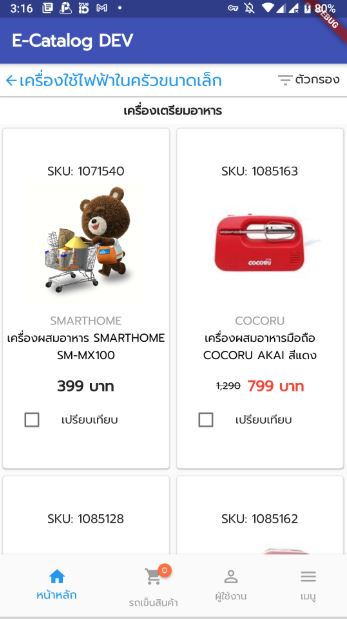
\includegraphics[width=0.35\textwidth]{compare1_1}
        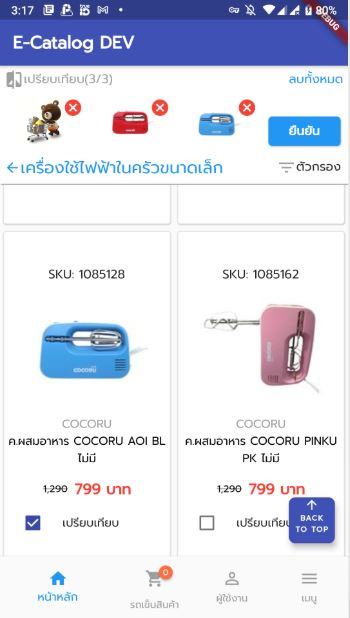
\includegraphics[width=0.35\textwidth]{compare1_2}
        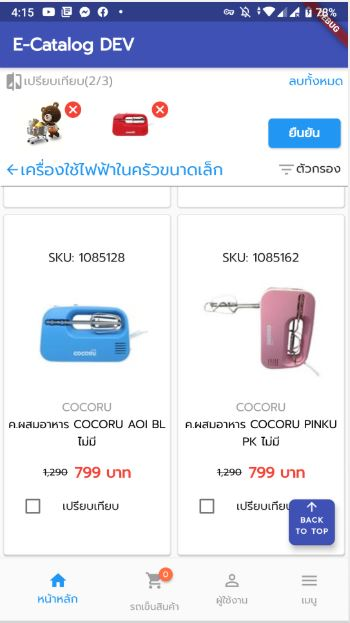
\includegraphics[width=0.35\textwidth]{delsome}
        \caption{ตัวอย่างเหตุการณ์ ยกเลิกตัวที่เปรียบเทียบบางรายการ}
        \label{Fig:36}
    \end{figure}

    \newpage
    \subsection{หน้าจอเปรียบเทียบสินค้า :ยกเลิกการเปรียบเทียบทั้งหมด}

    \begin{longtable}{|l|l|l|}
        \caption{ขอบเขตเหตุการณ์ยกเลิกการเปรียบเทียบทั้งหมด} \\ 
        \hline
        \textbf{ลำดับ} & \textbf{เหตุการณ์ในการทดสอบ} & \textbf{ผลลัพธ์ในการทดสอบ}  \endfirsthead 
        \hline
        1              & ทำการ Log-in               & PASS                        \\ 
        \hline
        2              & ไปยังหมวดหมู่ย่อย               & PASS                        \\ 
        \hline
        3              & กดเลือกปุ่มเปรียบเทียบสินค้า 3 ชิ้น       & PASS                        \\ 
        \hline
        4              & กดปุ่มลบทั้งหมดช่องเปรียบเทียบหาย    & PASS                        \\
        \hline
    \end{longtable}

    \begin{figure}[H]
        \centering
        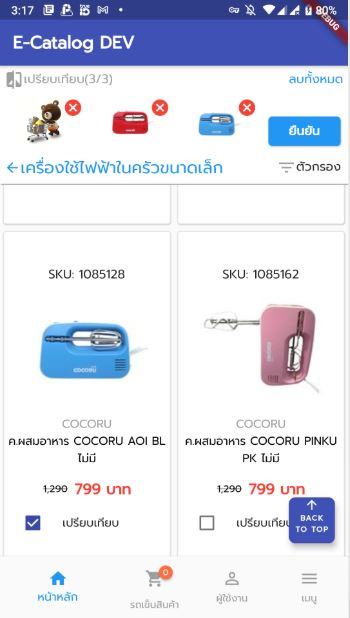
\includegraphics[width=0.35\textwidth]{compare1_2}
        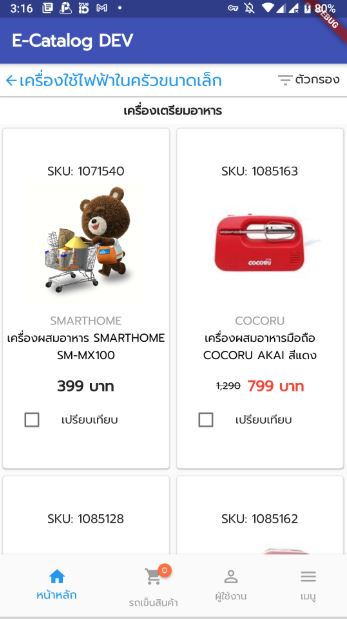
\includegraphics[width=0.35\textwidth]{compare1_1}
        \caption{ตัวอย่างเหตุการณ์ยกเลิกการเปรียบเทียบทั้งหมด}
        \label{Fig:37}
    \end{figure}

    \subsection{หน้าจอเปรียบเทียบสินค้า : ปุ่ม เพิ่มลงรถเข็น}

    \begin{longtable}{|l|l|l|}
        \caption{ขอบเขตเหตุการณ์ ปุ่ม เพิ่มลงรถเข็น} \\ 
        \hline
        \textbf{ลำดับ} & \textbf{เหตุการณ์ในการทดสอบ} & \textbf{ผลลัพธ์ในการทดสอบ}  \endfirsthead 
        \hline
        1              & ทำการ Log-in               & PASS                        \\ 
        \hline
        2              & ไปยังหมวดหมู่ย่อย               & PASS                        \\ 
        \hline
        3              & กดเลือกปุ่มเปรียบเทียบสินค้า 3 ชิ้น       & PASS                        \\ 
        \hline
        4              & กดยืนยันการเปรียบเทียบ     & PASS                        \\
        \hline
        5              & กดปุ่มใส่รถเข็น     & PASS                        \\
        \hline
        6              & สินค้าไปอยู่ในแถบรถเข็นสินค้า     & PASS                        \\
        \hline
    \end{longtable}

    \begin{figure}[H]
        \centering
        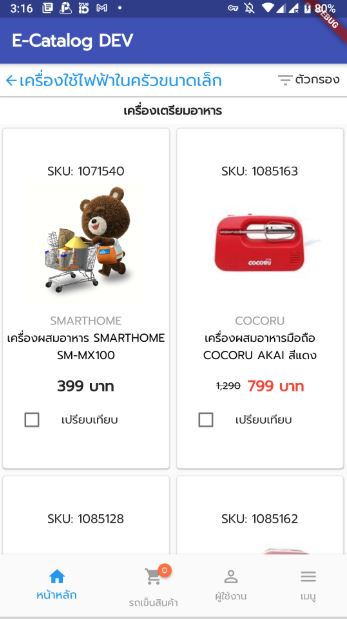
\includegraphics[width=0.35\textwidth]{compare1_1}
        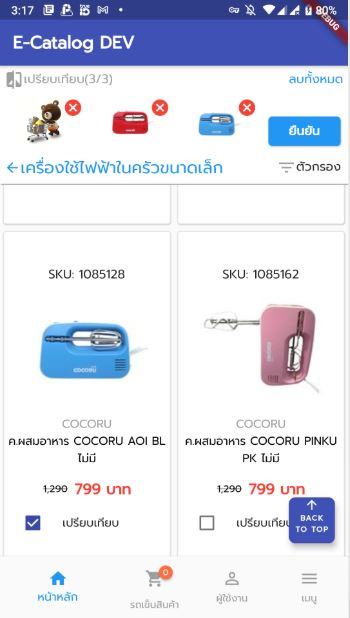
\includegraphics[width=0.35\textwidth]{compare1_2}
        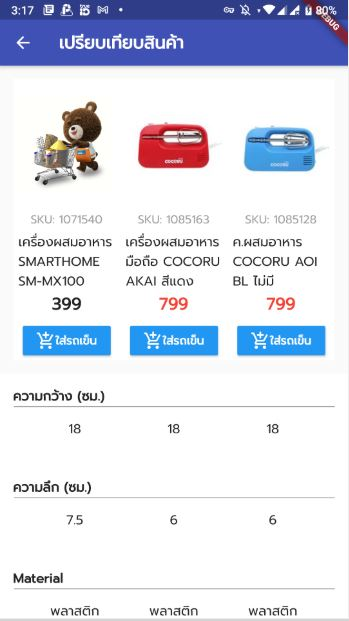
\includegraphics[width=0.35\textwidth]{compare1_3}
        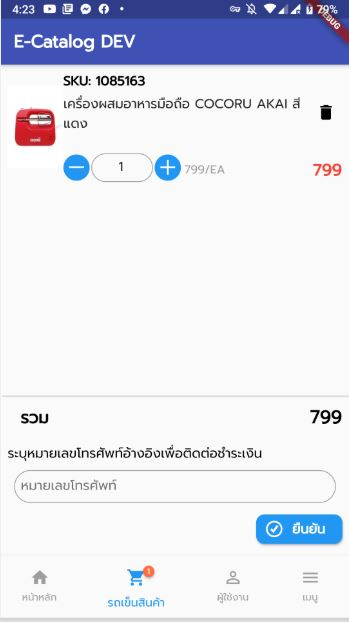
\includegraphics[width=0.35\textwidth]{compareCart}
        \caption{ตัวอย่างเหตุการณ์ ปุ่ม เพิ่มลงรถเข็น}
        \label{Fig:38}
    \end{figure}

    \subsection{รถเข็นสินค้า – แก้ไขรายการสินค้า : แก้ไขจำนวนสินค้า (เพิ่ม-ลด)}

    \begin{longtable}{|l|l|l|}
        \caption{ขอบเขตเหตุการณ์ รถเข็นสินค้า – แก้ไขรายการสินค้า แก้ไขจำนวนสินค้า (เพิ่ม-ลด)} \\ 
        \hline
        \textbf{ลำดับ} & \textbf{เหตุการณ์ในการทดสอบ} & \textbf{ผลลัพธ์ในการทดสอบ}  \endfirsthead 
        \hline
        1              & ทำการ Log-in               & PASS                        \\ 
        \hline
        2              & เลือกสินค้าใส่รถเข็น               & PASS                        \\ 
        \hline
        3              & ไปยังแถบ รถเข็นสินค้า       & PASS                        \\ 
        \hline
        4              & กดปุ่มเพิ่ม 2 ครั้ง     & PASS                        \\
        \hline
        5              & กดปุ่มลด 1 ครั้ง     & PASS                        \\
        \hline
        6              & เทียบจำนวนสินค้ากับเลขบนรูปรถเข็น     & PASS                        \\
        \hline
        7              & เทียบจำนวนสินค้ากับราคา     & PASS                        \\
        \hline
    \end{longtable}

    \begin{figure}[H]
        \centering
        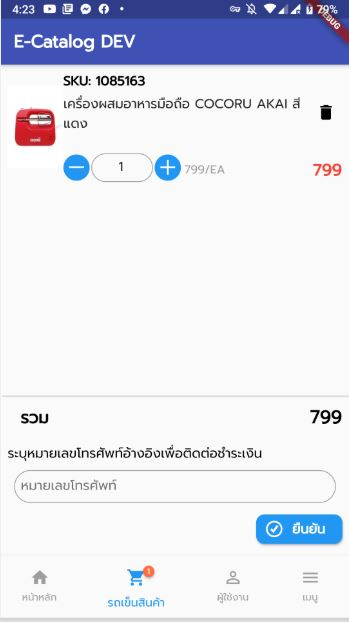
\includegraphics[width=0.35\textwidth]{compareCart}
        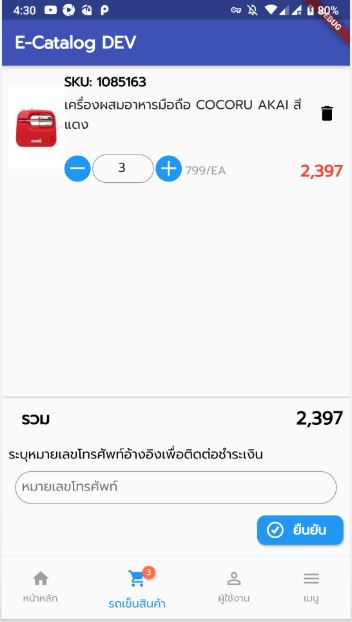
\includegraphics[width=0.35\textwidth]{cart1_1.JPG}
        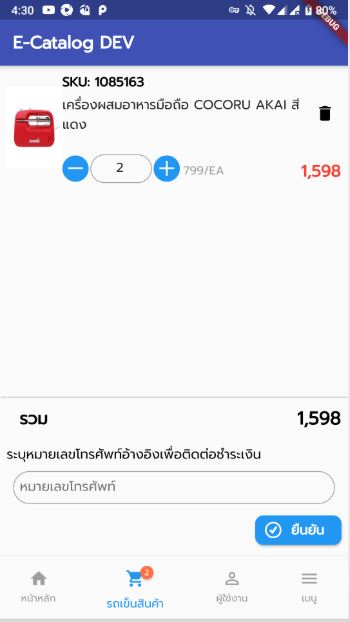
\includegraphics[width=0.35\textwidth]{cart1_2.JPG}
        \caption{ตัวอย่างเหตุการณ์ รถเข็นสินค้า – แก้ไขรายการสินค้า แก้ไขจำนวนสินค้า (เพิ่ม-ลด)}
        \label{Fig:39}
    \end{figure}

    \newpage
    \subsection{รถเข็นสินค้า – แก้ไขรายการสินค้า : แก้ไขจำนวนสินค้า (เพิ่ม) โดยให้มี QTY รวมกันเกิน 999}

    \begin{longtable}{|l|l|l|}
        \caption{ขอบเขตเหตุการณ์ รถเข็นสินค้า – แก้ไขรายการสินค้า แก้ไขจำนวนสินค้า (เพิ่ม) โดยให้มี QTY รวมกันเกิน 999} \\ 
        \hline
        \textbf{ลำดับ} & \textbf{เหตุการณ์ในการทดสอบ} & \textbf{ผลลัพธ์ในการทดสอบ}  \endfirsthead 
        \hline
        1              & ทำการ Log-in               & PASS                        \\ 
        \hline
        2              & เลือกสินค้าใส่รถเข็น 2 ชิ้น            & PASS                        \\ 
        \hline
        3              & ไปยังแถบ รถเข็นสินค้า       & PASS                        \\ 
        \hline
        4              & แก้จำนวนสินค้า 1 อันให้เกิน 999     & PASS                        \\
        \hline
        5              & ทียบจำนวนสินค้ากับเลขบนรูปรถเข็นว่าเป็น 999+ ไหม    & PASS                        \\
        \hline
        6              & เทียบจำนวนสินค้ากับราคาของ 999+ ชิ้น     & PASS                        \\
        \hline
    \end{longtable}

    \begin{figure}[H]
        \centering
        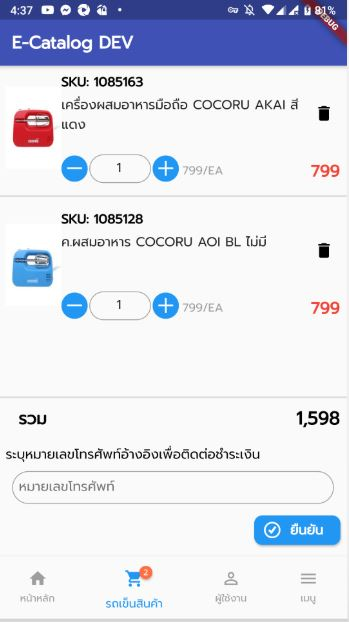
\includegraphics[width=0.35\textwidth]{cart2_1}
        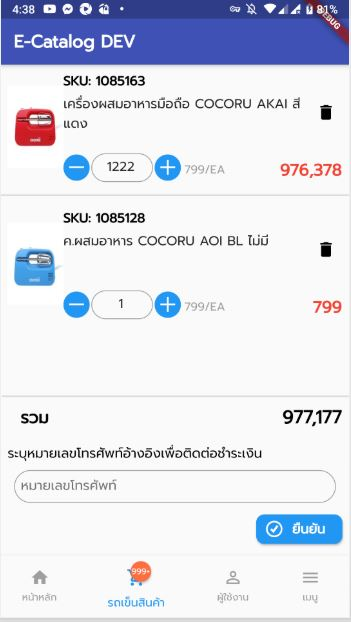
\includegraphics[width=0.35\textwidth]{cart2_2}
        \caption{ตัวอย่างเหตุการณ์ รถเข็นสินค้า – แก้ไขรายการสินค้า แก้ไขจำนวนสินค้า (เพิ่ม) โดยให้มี QTY รวมกันเกิน 999}
        \label{Fig:40}
    \end{figure}

    \newpage
    \subsection{รถเข็นสินค้า – แก้ไขรายการสินค้า : ลบรายการสินค้า}

    \begin{longtable}{|l|l|l|} 
        \caption{ขอบเขตเหตุการณ์ รถเข็นสินค้า – แก้ไขรายการสินค้า ลบรายการสินค้า} \\
        \hline
        \textbf{ลำดับ} & \textbf{เหตุการณ์ในการทดสอบ} & \textbf{ผลลัพธ์ในการทดสอบ}  \endfirsthead 
        \hline
        1              & ทำการ Log-in               & PASS                        \\ 
        \hline
        2              & เลือกสินค้าใส่รถเข็น 2 ชิ้น            & PASS                        \\ 
        \hline
        3              & ไปยังแถบ รถเข็นสินค้า       & PASS                        \\ 
        \hline
        4              & แก้จำนวนสินค้า 1 อันให้เกิน 999     & PASS                        \\
        \hline
        5              & ลบสินค้า 1 ชิ้น    & PASS                        \\
        \hline
        6              & เทียบจำนวนสินค้ากับเลขบนรูปรถเข็นลดลงจากที่ลบหรือไม่     & PASS                        \\
        \hline
        7              & เทียบราคาสินค้าว่าลดลงหรือไม่     & PASS                        \\
        \hline
    \end{longtable}

    \begin{figure}[H]
        \centering
        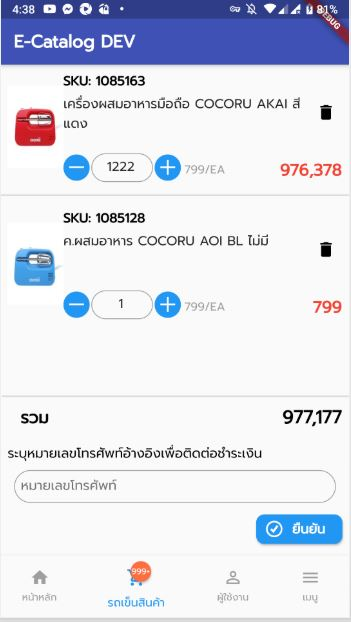
\includegraphics[width=0.35\textwidth]{cart2_2}
        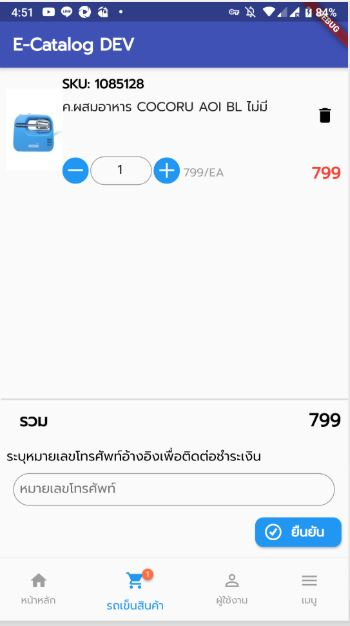
\includegraphics[width=0.35\textwidth]{delcart}
        \caption{ตัวอย่างเหตุการณ์ รถเข็นสินค้า – แก้ไขรายการสินค้า ลบรายการสินค้า}
        \label{Fig:42}
    \end{figure}

    \newpage
    \subsection{รถเข็นสินค้า – สร้างใบคำสั่งซื้อ : สร้างใบคำสั่งซื้อ โดยใช้เบอร์โทรที่ไม่ใช่เบอร์มือถือ}

    \begin{longtable}{|l|l|l|} 
        \caption{ขอบเขตเหตุการณ์ รถเข็นสินค้า – สร้างใบคำสั่งซื้อ สร้างใบคำสั่งซื้อ โดยใช้เบอร์โทรที่ไม่ใช่เบอร์มือถือ} \\
        \hline
        \textbf{ลำดับ} & \textbf{เหตุการณ์ในการทดสอบ} & \textbf{ผลลัพธ์ในการทดสอบ}  \endfirsthead 
        \hline
        1              & ทำการ Log-in               & PASS                        \\ 
        \hline
        2              & เลือกสินค้าใส่รถเข็น 1 ชิ้น            & PASS                        \\ 
        \hline
        3              & ไปยังแถบ รถเข็นสินค้า       & PASS                        \\ 
        \hline
        4              & กรอกเบอร์โทรศพท์บ้าน     & PASS                        \\
        \hline
        5              & แจ้งเตือนแสดงว่าไม่ผ่าน     & PASS                        \\
        \hline
    \end{longtable}

    \begin{figure}[H]
        \centering
        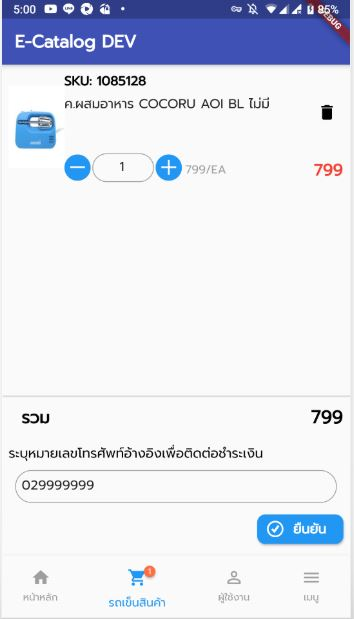
\includegraphics[width=0.35\textwidth]{order1_2}
        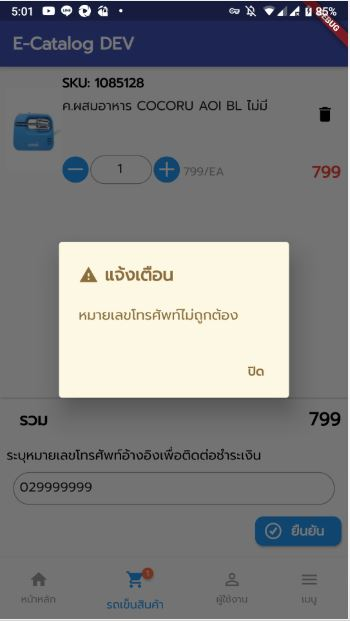
\includegraphics[width=0.35\textwidth]{order1_3}
        \caption{ตัวอย่างเหตุการณ์ รถเข็นสินค้า – สร้างใบคำสั่งซื้อ สร้างใบคำสั่งซื้อ โดยใช้เบอร์โทรที่ไม่ใช่เบอร์มือถือ}
        \label{Fig:43}
    \end{figure}

    \newpage
    \subsection{รถเข็นสินค้า – สร้างใบคำสั่งซื้อ : สร้างใบคำสั่งซื้อ โดยใช้เบอร์โทรที่เบอร์มือถือถูกต้อง}

    \begin{longtable}{|l|l|l|} 
        \caption{ขอบเขตเหตุการณ์ รถเข็นสินค้า – สร้างใบคำสั่งซื้อ สร้างใบคำสั่งซื้อ โดยใช้เบอร์โทรที่เบอร์มือถือถูกต้อง} \\
        \hline
        \textbf{ลำดับ} & \textbf{เหตุการณ์ในการทดสอบ} & \textbf{ผลลัพธ์ในการทดสอบ}  \endfirsthead 
        \hline
        1              & ทำการ Log-in               & PASS                        \\ 
        \hline
        2              & เลือกสินค้าใส่รถเข็น 1 ชิ้น            & PASS                        \\ 
        \hline
        3              & ไปยังแถบ รถเข็นสินค้า       & PASS                        \\ 
        \hline
        4              & กรอกเบอร์โทรศพท์มือถือ     & PASS                        \\
        \hline
        5              & แจ้งเตือนแสดงว่าผ่าน     & PASS                        \\
        \hline
    \end{longtable}

    \begin{figure}[H]
        \centering
        \includegraphics[width=0.35\textwidth]{order2_2}
        \includegraphics[width=0.35\textwidth]{order2_3}
        \caption{ตัวอย่างเหตุการณ์ รถเข็นสินค้า – สร้างใบคำสั่งซื้อ สร้างใบคำสั่งซื้อ โดยใช้เบอร์โทรที่เบอร์มือถือถูกต้อง}
        \label{Fig:44}
    \end{figure}

    \newpage
    \subsection{ผู้ใช้งาน : ข้อมูลผู้เข้าใช้งาน}

    \begin{longtable}{|l|l|l|} 
        \caption{ขอบเขตเหตุการณ์ ผู้ใช้งาน ข้อมูลผู้เข้าใช้งาน} \\
        \hline
        \textbf{ลำดับ} & \textbf{เหตุการณ์ในการทดสอบ} & \textbf{ผลลัพธ์ในการทดสอบ}  \endfirsthead 
        \hline
        1              & ทำการ Log-in               & PASS                        \\ 
        \hline
        2              & กดไปที่ปุ่มผู้ใช้งาน                & PASS                        \\ 
        \hline
        3              & เช็ค EMP ID                & PASS                        \\ 
        \hline
        4              & เช็ค EMP Name     & PASS                        \\
        \hline
        5              & เช็ค Transaction Date     & PASS                        \\
        \hline
        6              & เช็ค EMP สาขาที่ขาย     & PASS                        \\
        \hline
    \end{longtable}

    \begin{figure}[H]
        \centering
        \includegraphics[width=0.35\textwidth]{user1}
        \includegraphics[width=0.35\textwidth]{user1_2}
        \caption{ตัวอย่างเหตุการณ์ ผู้ใช้งาน ข้อมูลผู้เข้าใช้งาน}
        \label{Fig:45}
    \end{figure}

    % เกิด Error ตั้งแต่ตรงนี้

    \newpage
    \subsection{เมนู – เลือกหมวดสินค้า : การค้นหาสินค้าจากการเลือกหมวดสินค้า}

    \begin{longtable}{|l|l|l|} 
        \caption{ขอบเขตเหตุการณ์ เมนู – เลือกหมวดสินค้า การค้นหาสินค้าจากการเลือกหมวดสินค้า} \\
        \hline
        \textbf{ลำดับ} & \textbf{เหตุการณ์ในการทดสอบ} & \textbf{ผลลัพธ์ในการทดสอบ}  \endfirsthead 
        \hline
        1              & ทำการ Log-in               & PASS                        \\ 
        \hline
        2              & กดไปที่ปุ่มเมนู               & PASS                        \\ 
        \hline
        3              & กดไปเลือกหมวดสินค้า                & PASS                        \\ 
        \hline
        4              & เลือกหมวดเครื่องใช้ไฟฟ้า     & PASS                        \\
        \hline
        5              & เช็ค ว่ามีหลอดไฟที่เป็นเครื่องใช้ไฟฟ้าหรือไม่     & PASS                        \\
        \hline
    \end{longtable}

    \begin{figure}[H]
        \centering
        \includegraphics[width=0.35\textwidth]{logout2}
        \includegraphics[width=0.35\textwidth]{logout2_1}
        \caption{ตัวอย่างเหตุการณ์ เมนู – เลือกหมวดสินค้า การค้นหาสินค้าจากการเลือกหมวดสินค้า}
        \label{Fig:46}
    \end{figure}


    \newpage
    \subsection{เมนู – เลือกหมวดสินค้า : การค้นหาสินค้าจากการเลือกแบรนด์สินค้า}

    \begin{longtable}{|l|l|l|}
        \caption{ขอบเขตเหตุการณ์ เมนู – เลือกหมวดสินค้า การค้นหาสินค้าจากการเลือกแบรนด์สินค้า} \\
        \hline
        \textbf{ลำดับ} & \textbf{เหตุการณ์ในการทดสอบ} & \textbf{ผลลัพธ์ในการทดสอบ}  \endfirsthead 
        \hline
        1              & ทำการ Log-in               & PASS                        \\ 
        \hline
        2              & กดไปที่ปุ่มเมนู               & PASS                        \\ 
        \hline
        3              & กดไปเลือกแบรนสินค้า                & PASS                        \\ 
        \hline
        4              & เลือกแบรน ALLUSION     & PASS                        \\
        \hline
        5              & เช็คว่ามีแบรน ALLUSION     & PASS                        \\
        \hline
    \end{longtable}

    \begin{figure}[H]
        \centering
        \includegraphics[width=0.35\textwidth]{brand1_1.JPG}
        \includegraphics[width=0.35\textwidth]{brand1_2.JPG}
        \caption{ตัวอย่างเหตุการณ์ เมนู – เลือกหมวดสินค้า การค้นหาสินค้าจากการเลือกแบรนด์สินค้า}
        \label{Fig:47}
    \end{figure}

    \newpage
    \subsection{เมนู – ภาษา : การเลือกภาษา}

    \begin{longtable}{|l|l|l|}
        \caption{ขอบเขตเหตุการณ์ เมนู – ภาษา การเลือกภาษา} \\
        \hline
        \textbf{ลำดับ} & \textbf{เหตุการณ์ในการทดสอบ} & \textbf{ผลลัพธ์ในการทดสอบ}  \endfirsthead 
        \hline
        1              & ทำการ Log-in               & PASS                        \\ 
        \hline
        2              & กดไปที่ปุ่มเมนู               & PASS                        \\ 
        \hline
        3              & กดไปเลือกที่เปลี่ยนภาษา                & PASS                        \\ 
        \hline
        4              & เลือกภาษาอังกฤษ     & PASS                        \\
        \hline
        5              & เช็คตัวภาษาด้านบนเปลี่ยนหรือไม่     & PASS                        \\
        \hline
    \end{longtable}

    \begin{figure}[H]
        \centering
        \includegraphics[width=0.35\textwidth]{lang1}
        \includegraphics[width=0.35\textwidth]{lang2}
        \caption{ตัวอย่างเหตุการณ์ เมนู – ภาษา การเลือกภาษา}
        \label{Fig:48}
    \end{figure}

    \subsection{หน้าหลัก - หมวดหมู่หลัก (Level 3) : ปุ่มค้นหา}
    วิธีนี้เลือกใช้การใช้กับ Driver Wd เนื่องจากต้องให้อุปกรณ์แสดงคีย์บอร์ดในการพิมพ์เพื่อ submit การค้นหาด้วย PressKeycode
    \begin{longtable}{|l|l|l|}
        \caption{ขอบเขตเหตุการณ์ หมวดหมู่หลัก (Level 3) ปุ่มค้นหา} \\
        \hline
        \textbf{ลำดับ} & \textbf{เหตุการณ์ในการทดสอบ} & \textbf{ผลลัพธ์ในการทดสอบ}  \endfirsthead 
        \hline
        1              & ทำการ Log-in               & PASS                        \\ 
        \hline
        2              & กดปุ่มและค้นหาสินค้า               & PASS                        \\ 
        \hline
        3              & แสดงสินค้ารหัส 255255               & PASS                        \\ 
        \hline
    \end{longtable}

    \begin{figure}[H]
        \centering
        \includegraphics[width=0.35\textwidth]{search}
        \includegraphics[width=0.35\textwidth]{search2}
        \caption{ตัวอย่างเหตุการณ์ หมวดหมู่หลัก (Level 3) ปุ่มค้นหา}
        \label{Fig:60}
    \end{figure}

\section{ผลการทดสอบด้วยการจับ แก้ไขที่ Source Code ของ Flutter โดยใช้ Appium Flutter Driver}
เป็นวิธีการทดสอบโดยการจับ Element กับแอปพลิเคชันที่ถูกสร้างด้วย Flutter ซึ่งต้องแก้ไขตัว Source Code ของแอปพลิเคชันโดยการใส่ Key ใน Element ที่จะจับดังตัวอย่างด้านล่าง 
\begin{figure}[H]
    \centering
    \includegraphics[width=1\textwidth]{keyAdd}
    \caption{ตัวอย่างการเพิ่ม Key กับ Element}\label{keyAdd}
\end{figure}

จากรูปที่ 3.30 เป็นการเพิ่ม Key ใน Element ของปุ่มซึ่งสามารถนำมาเรียกใช้ในการจับได้แต่ก็มีข้อจำกัดในบาง Element เช่น SlideBar เป็นต้นเนื่องจากจะจับตัวลากไม่ได้เลือก
 ใช้วิธีนี้เมื่อลำดับของ Element เปลี่ยนทำให้แบบไม่แก้ Source Code ไม่แน่นอน

\begin{figure}[H]
    \centering
    \includegraphics[width=1\textwidth]{resultFlutter}
    \includegraphics[width=1\textwidth]{resultFail}
    \caption{ตัวอย่างการแสดงผลการทดสอบแบบผ่านและมีข้อผิดพลาด}\label{keyAdd1}
\end{figure}

จากรูป 3.31 เป็นตัวอย่างการทดสอบหากผ่านการทดสอบและหากพบข้อผิดพลาดจะแสดงผลอย่างไร

\begin{longtable}{|l|l|}
    \caption{ตารางข้อเปรียบเทียบการทดสอบด้วยการจับ แก้ไขที่ Source Code ของ Flutter โดยใช้ Appium Flutter Driver}\\ 
    \hline
    \textbf{ข้อดี}  & \textbf{ข้อเสีย} \endfirsthead 
    \hline
    \begin{tabular}[c]{@{}l@{}}สามารถจับ Element ได้แม่นยำตาม\\key ที่ developer สร้างเอาไว้\end{tabular}                                                                      & \begin{tabular}[c]{@{}l@{}}ไม่สามารถแสดงคีย์บอร์ดที่เปรียบเสมือน\\การพิมพ์ได้ทำให้ไม่สามารถทดสอบบาง\\~function ได้\end{tabular}  \\ 
    \hline
    \begin{tabular}[c]{@{}l@{}}สามารถใช้ Flutter\_Driver ที่เป็นตัวทดสอบ\\~แอปพลิเคชันที่สร้างด้วย Flutter ที่ปกติเขียนด้วย \\Dart สามารถนำมาเขียนเป็นภาษาอื่นได้\end{tabular} & \begin{tabular}[c]{@{}l@{}}ต้องไปแก้ที่ Source Code และ \\build ใหม่เสมอเมื่อต้องการนำมาทดสอบ\end{tabular}                       \\ 
    \hline
                                                                                                                                                                               & \begin{tabular}[c]{@{}l@{}}ยังไม่สามารถนำ Flutter\_Driver \\มาใช้ได้อย่างสมบูรณ์เพราะพัฒนาไม่เสร็จ\end{tabular}                  \\
    \hline
\end{longtable}

    \newpage
    \subsection{หน้าหลัก - หมวดหมู่หลัก (Level 3) : ตรวจสอบการแสดงหมวดหมู่สินค้า}
    \begin{longtable}{|l|l|l|}
        \caption{ขอบเขตเหตุการณ์ หมวดหมู่หลัก (Level 3) ตรวจสอบการแสดงหมวดหมู่สินค้า} \\
        \hline
        \textbf{ลำดับ} & \textbf{เหตุการณ์ในการทดสอบ} & \textbf{ผลลัพธ์ในการทดสอบ}  \endfirsthead 
        \hline
        1              & ทำการ Log-in               & PASS                        \\ 
        \hline
        2              & เช็คชื่อหมวดทั้ง 16 หมวด               & PASS                        \\ 
        \hline
    \end{longtable}

    \begin{figure}[H]
        \centering
        \includegraphics[width=0.35\textwidth]{level3_1}
        \includegraphics[width=0.35\textwidth]{level3_2}
        \caption{ตัวอย่างเหตุการณ์ หมวดหมู่หลัก (Level 3) ตรวจสอบการแสดงหมวดหมู่สินค้า}
        \label{Fig:75}
    \end{figure}

    \newpage
    \subsection{หน้าหลัก - หมวดหมู่ย่อย (Level 2) : ตรวจสอบการแสดงหมวดหมู่สินค้า}
    \begin{longtable}{|l|l|l|}
        \caption{ขอบเขตเหตุการณ์ หมวดหมู่ย่อย (Level 2) ตรวจสอบการแสดงหมวดหมู่สินค้า} \\
        \hline
        \textbf{ลำดับ} & \textbf{เหตุการณ์ในการทดสอบ} & \textbf{ผลลัพธ์ในการทดสอบ}  \endfirsthead 
        \hline
        1              & ทำการ Log-in               & PASS                        \\ 
        \hline
        2              & กดเข้าทีละหมวด (level 3)             & PASS                        \\ 
        \hline
        3              & เช็คชื่อหมวดย่อย (level 2)               & PASS                        \\ 
        \hline
    \end{longtable}

    \begin{figure}[H]
        \centering
        \includegraphics[width=0.35\textwidth]{level2_1_1}
        \includegraphics[width=0.35\textwidth]{level2_1_2}
        \includegraphics[width=0.35\textwidth]{level2_1_3}
        \caption{ตัวอย่างเหตุการณ์ หมวดหมู่ย่อย (Level 2) ตรวจสอบการแสดงหมวดหมู่สินค้า}
        \label{Fig:61}
    \end{figure}

    \newpage
    \subsection{หน้าหลัก - หมวดหมู่ย่อย (Level 2) : ดูทั้งหมด}
    \begin{longtable}{|l|l|l|}
        \caption{ขอบเขตเหตุการณ์ หมวดหมู่ย่อย (Level 2) ดูทั้งหมด} \\
        \hline
        \textbf{ลำดับ} & \textbf{เหตุการณ์ในการทดสอบ} & \textbf{ผลลัพธ์ในการทดสอบ}  \endfirsthead 
        \hline
        1              & ทำการ Log-in               & PASS                        \\ 
        \hline
        2              & กดเข้าทีละหมวด (level 3)             & PASS                        \\ 
        \hline
        3              & กดปุ่มดูทั้งหมด (level 2)               & PASS                        \\ 
        \hline
        4              & เช็คการแสดงผลว่าตรงกับหมวดที่กดไหม (level 2)               & PASS                        \\ 
        \hline
    \end{longtable}

    \begin{figure}[H]
        \centering
        \includegraphics[width=0.35\textwidth]{level2_2_1}
        \includegraphics[width=0.35\textwidth]{level2_2_2}
        \caption{ตัวอย่างเหตุการณ์ หมวดหมู่ย่อย (Level 2) ดูทั้งหมด}
        \label{Fig:62}
    \end{figure}

    \newpage
    \subsection{หน้าหลัก - หมวดหมู่ย่อย (Level 1) : เลือกตัวกรอง – ตัวกรองหมวดสินค้า}
    \begin{longtable}{|l|l|l|}
        \caption{ขอบเขตเหตุการณ์ หมวดหมู่ย่อย (Level 1) เลือกตัวกรอง – ตัวกรองหมวดสินค้า} \\
        \hline
        \textbf{ลำดับ} & \textbf{เหตุการณ์ในการทดสอบ} & \textbf{ผลลัพธ์ในการทดสอบ}  \endfirsthead 
        \hline
        1              & ทำการ Log-in               & PASS                        \\ 
        \hline
        2              & กดเข้าหมวดกีฬา             & PASS                        \\ 
        \hline
        3              & กดปุ่มดูทั้งหมด (level 2)               & PASS                        \\ 
        \hline
        4              & กดสัญลักษณ์ปุ่ม filter               & PASS                        \\ 
        \hline
        5              & เลือกหมวดสินค้า              & PASS                        \\ 
        \hline
        6              & เช็คสินค้าว่าตรงกับหมวด              & PASS                        \\ 
        \hline
    \end{longtable}

    \begin{figure}[H]
        \centering
        \includegraphics[width=0.35\textwidth]{level1_1_2}
        \includegraphics[width=0.35\textwidth]{level1_1_3}
        \caption{ตัวอย่างเหตุการณ์ หมวดหมู่ย่อย (Level 1) เลือกตัวกรอง – ตัวกรองหมวดสินค้า}
        \label{Fig:70}
    \end{figure}

    \newpage
    \subsection{หน้าหลัก - หมวดหมู่ย่อย (Level 1) : เลือกตัวกรอง – ตัวกรองแบรนด์}
    \begin{longtable}{|l|l|l|}
        \caption{ขอบเขตเหตุการณ์ หมวดหมู่ย่อย (Level 1) เลือกตัวกรอง – ตัวกรองแบรนด์} \\
        \hline
        \textbf{ลำดับ} & \textbf{เหตุการณ์ในการทดสอบ} & \textbf{ผลลัพธ์ในการทดสอบ}  \endfirsthead 
        \hline
        1              & ทำการ Log-in               & PASS                        \\ 
        \hline
        2              & กดเข้าหมวดกีฬา             & PASS                        \\ 
        \hline
        3              & กดปุ่มดูทั้งหมด (level 2)               & PASS                        \\ 
        \hline
        4              & กดสัญลักษณ์ปุ่ม filter               & PASS                        \\ 
        \hline
        5              & เลือกแบรนด์              & PASS                        \\ 
        \hline
        6              & เช็คสินค้าว่าตรงกับแบรนด์ที่เลือก              & PASS                        \\ 
        \hline
    \end{longtable}

    \begin{figure}[H]
        \centering
        \includegraphics[width=0.35\textwidth]{level1_2_2}
        \includegraphics[width=0.35\textwidth]{level1_2_3}
        \caption{ตัวอย่างเหตุการณ์ หมวดหมู่ย่อย (Level 1) เลือกตัวกรอง – ตัวกรองแบรนด์}
        \label{Fig:63}
    \end{figure}

    \newpage
    \subsection{หน้าหลัก - หมวดหมู่ย่อย (Level 1) : ตรวจสอบการแสดงหมวดหมู่สินค้า Default}
    \begin{longtable}{|l|l|l|}
        \caption{ขอบเขตเหตุการณ์ หมวดหมู่ย่อย (Level 1) ตรวจสอบการแสดงหมวดหมู่สินค้า Default} \\
        \hline
        \textbf{ลำดับ} & \textbf{เหตุการณ์ในการทดสอบ} & \textbf{ผลลัพธ์ในการทดสอบ}  \endfirsthead 
        \hline
        1              & ทำการ Log-in               & PASS                        \\ 
        \hline
        2              & กดเข้าหมวดกีฬา             & PASS                        \\ 
        \hline
        3              & กดปุ่มดูทั้งหมด (level 2)               & PASS                        \\ 
        \hline
        4              & เช็คสินค้าว่าเรียงราคาจากน้อยไปมากตาม Default              & PASS                        \\ 
        \hline
    \end{longtable}

    \begin{figure}[H]
        \centering
        \includegraphics[width=0.35\textwidth]{level1_1_1}
        \includegraphics[width=0.35\textwidth]{level1_default}
        \caption{ตัวอย่างเหตุการณ์ หมวดหมู่ย่อย (Level 1) ตรวจสอบการแสดงหมวดหมู่สินค้า Default}
        \label{Fig:64}
    \end{figure}

    \newpage
    \subsection{หน้าหลัก - หมวดหมู่ย่อย (Level 1) : ตัวเลือก จัดเรียง – เรียงจากราคาน้อยไปหามาก}
    \begin{longtable}{|l|l|l|}
        \caption{ขอบเขตเหตุการณ์ หมวดหมู่ย่อย (Level 1) ตัวเลือก จัดเรียง – เรียงจากราคาน้อยไปหามาก} \\
        \hline
        \textbf{ลำดับ} & \textbf{เหตุการณ์ในการทดสอบ} & \textbf{ผลลัพธ์ในการทดสอบ}  \endfirsthead 
        \hline
        1              & ทำการ Log-in               & PASS                        \\ 
        \hline
        2              & กดเข้าหมวดกีฬา             & PASS                        \\ 
        \hline
        3              & กดปุ่มดูทั้งหมด (level 2)               & PASS                        \\ 
        \hline
        4              & กดสัญลักษณ์ปุ่ม filter               & PASS                        \\ 
        \hline
        5              & กดที่แถบเรียงตาม              & PASS                        \\ 
        \hline
        6              & เลือกราคาน้อยไปมาก              & PASS                        \\ 
        \hline
        7              & เช็คสินค้าเรียงราคาน้อยไปหามาก              & PASS                        \\ 
        \hline
    \end{longtable}

    \begin{figure}[H]
        \centering
        \includegraphics[width=0.35\textwidth]{level_less}
        \includegraphics[width=0.35\textwidth]{level_less2}
        \caption{ตัวอย่างเหตุการณ์ หมวดหมู่ย่อย (Level 1) ตัวเลือก จัดเรียง – เรียงจากราคาน้อยไปหามาก}
        \label{Fig:65}
    \end{figure}

    \newpage
    \subsection{หน้าหลัก - หมวดหมู่ย่อย (Level 1) : ตัวเลือก จัดเรียง – เรียงจากราคามากไปหาน้อย}
    \begin{longtable}{|l|l|l|}
        \caption{ขอบเขตเหตุการณ์ หมวดหมู่ย่อย (Level 1) ตัวเลือก จัดเรียง – เรียงจากราคามากไปหาน้อย} \\
        \hline
        \textbf{ลำดับ} & \textbf{เหตุการณ์ในการทดสอบ} & \textbf{ผลลัพธ์ในการทดสอบ}  \endfirsthead 
        \hline
        \textbf{ลำดับ} & \textbf{เหตุการณ์ในการทดสอบ} & \textbf{ผลลัพธ์ในการทดสอบ}  \endfirsthead 
        \hline
        1              & ทำการ Log-in               & PASS                        \\ 
        \hline
        2              & กดเข้าหมวดกีฬา             & PASS                        \\ 
        \hline
        3              & กดปุ่มดูทั้งหมด (level 2)               & PASS                        \\ 
        \hline
        4              & กดสัญลักษณ์ปุ่ม filter               & PASS                        \\ 
        \hline
        5              & กดที่แถบเรียงตาม              & PASS                        \\ 
        \hline
        6              & เลือกราคามากไปน้อย              & PASS                        \\ 
        \hline
        7              & เช็คสินค้าเรียงราคามากไปหาน้อย              & PASS                        \\ 
        \hline
    \end{longtable}

    \begin{figure}[H]
        \centering
        \includegraphics[width=0.35\textwidth]{level_more1}
        \includegraphics[width=0.35\textwidth]{level_more2}
        \caption{ตัวอย่างเหตุการณ์ หมวดหมู่ย่อย (Level 1) ตัวเลือก จัดเรียง – เรียงจากราคามากไปหาน้อย}
        \label{Fig:66}
    \end{figure}

    \newpage
    \subsection{หน้าหลัก - หมวดหมู่ย่อย (Level 1) : ตัวเลือก เปรียบสินค้าหน้าหลัก}
    \begin{longtable}{|l|l|l|}
        \caption{ขอบเขตเหตุการณ์ หมวดหมู่ย่อย (Level 1) ตัวเลือก เปรียบสินค้าหน้าหลัก} \\
        \hline
        \textbf{ลำดับ} & \textbf{เหตุการณ์ในการทดสอบ} & \textbf{ผลลัพธ์ในการทดสอบ}  \endfirsthead 
        \hline
        \textbf{ลำดับ} & \textbf{เหตุการณ์ในการทดสอบ} & \textbf{ผลลัพธ์ในการทดสอบ}  \endfirsthead 
        \hline
        1              & ทำการ Log-in               & PASS                        \\ 
        \hline
        2              & กดเข้าหมวดกีฬา             & PASS                        \\ 
        \hline
        3              & กดปุ่มดูทั้งหมด (level 2)               & PASS                        \\ 
        \hline
        4              & กดปุ่มเปรียบเทียบ 2 อัน             & PASS                        \\ 
        \hline
        5              & สินค้า 2 ชิ้นอยู่แถบเปรียบเทียบ              & PASS                        \\ 
        \hline
    \end{longtable}

    \begin{figure}[H]
        \centering
        \includegraphics[width=0.35\textwidth]{level1_1_1}
        \includegraphics[width=0.35\textwidth]{level1_compare}
        \caption{ตัวอย่างเหตุการณ์ หมวดหมู่ย่อย (Level 1) ตัวเลือก เปรียบสินค้าหน้าหลัก}
        \label{Fig:67}
    \end{figure}

\newpage
\section{ผลการทดสอบด้วยการใช้ AWS Device Farm}
การใช้ AWS Device Farm ใช้เพื่อลดเวลาในการทดสอบและความหลากหลายของอุปกรณ์ในการทดสอบ

\begin{figure}[H]
    \centering
    \includegraphics[width=1\textwidth]{devicefram1}
    \includegraphics[width=1\textwidth]{devicefarm2}
    \caption{ตัวอย่างผลการทดลองนำไปทดสอบบน AWS Device Farm}
    \label{Fig:90}
\end{figure}

จากรูป 3.42 ค้นพบว่าการทดสอบบน AWS Device Farm กับแอปพลิเคชัน HomePro E-Catalog ไม่สามารถทำได้เพราะแอปพลิเคชันนี้รองรับในการใช้กับอินเทอร์เน็ตภายในองค์กรเท่านั้น


\begin{figure}[H]
    \centering
    \includegraphics[width=0.35\textwidth]{test1}
    \includegraphics[width=0.35\textwidth]{test2}
    \includegraphics[width=0.35\textwidth]{test3}
    \includegraphics[width=0.35\textwidth]{test4}
    \caption{ตัวอย่างภาพบันทึกหน้าจอจาก AWS Devices Faem}
    \label{Fig:90}
\end{figure}

จากรูป 3.42 คือรูปที่เกิดจากการบันทึกหน้าจอจาก AWS Device Farm ตอนทำการทดสอบและแสดงว่าไม่สามารถทดสอบได้

\subsection{แนวทางการแก้ปัญหา}
การแก้ปัญหาคือการที่จะต้องสร้าง Amazon Virtual Private Cloud ซึ่งจะต้องมีค่าใช้จ่ายในการทำเพื่อที่จะสามารถเชื่อมต่อกับอินเทอร์เน็ตภายในองค์กรได้แต่ทางองค์กรไม่ได้จัดสรรส่วนนี้ให้ในการทำการทดสอบทำให้ไม่สามารถนำ ชุดคำสั่งทดสอบ แอปพลิเคชัน HomePro E-Catalog ไปทดสอบบน AWS Devices Farm ได้


\section{ประโยชน์ที่ได้รับจากปฏิบัติงานสหกิจศึกษา}
ได้พัฒนาทักษะในด้านการทำชุดคำสั่งทดสอบอัตโนมัติ (Automate Test) ซึ่งเป็นทักษะที่ทางคณะไม่เคยมีอยู่ในหลักสูตรและไม่เคยทำมาก่อนจึงเป็นเรื่องท้าทายในการหาข้อมูลและนำมาประยุกต์ใช้อีกทั้งยังได้ฝึกทักษะในการแก้ปัญหาโปรแกรมต่างๆขนาดใหญ่ที่ทางบริษัทนำมาให้แก้เป็นงานนอกเหนือจากทำชุดคำสั่งทดสอบอัตโนมัติทำให้ได้เรียนรู้ว่าการทำงานจริงส่วนใหญ่คือการพัฒนาของเดิมให้ดีขึ้นไม่ใช่การสร้างใหม่